\section{Computational Modeling of $\beta$-secretase 1 (BACE-1) Inhibitors using Ligand Based Approaches}

This chapter is adapted from: 

Govindan Subramanian, Bharath Ramsundar, Vijay Pande, and Rajiah Aldrin Denny. "Computational modeling of β-secretase 1 (BACE-1) inhibitors using ligand based approaches." Journal of chemical information and modeling. \cite{subramanian2016computational}.

I was the second author and worked on conception of the original idea, implementation and execution of machine learning experiments, and writing of the paper.

\subsection{Abstract}
The binding affinities (IC50) reported for diverse structural and chemical classes of human $\beta$-secretase 1 (BACE-1) inhibitors in literature were modeled using multiple in silico ligand based modeling approaches and statistical techniques.  The descriptor space encompasses simple binary molecular fingerprint, 1- and 2-dimensional constitutional, physicochemical and topological descriptors, and sophisticated 3-dimensional molecular fields that require appropriate structural alignments of varied chemical scaffolds in one universal chemical space.  The affinities were modeled using qualitative classification or quantitative regression schemes involving linear, non-linear, and deep neural network (DNN) machine-learning methods used in the scientific literature for quantitative structure activity relationships (QSAR).  In a departure from tradition, ~20\% of the chemically diverse dataset (205 compounds) was used to train the model with the remaining ~80\% of the structural and chemical analogs used as part of an external validation (1273 compounds) and prospective test (69 compounds) sets respectively to ascertain the model performance.  The machine learning methods investigated herein performed well in both the qualitative classification (~70\% accuracy) and quantitative IC50 predictions (RMSE ~ 1 log).  The success of the 2D descriptor based machine learning approach when compared against the 3D field based technique pursued for hBACE-1 inhibitors provides a strong impetus for systematically applying such methods during the lead identification and optimization efforts for other protein families as well.


\subsection{Introduction}

In silico computer assisted drug design (CADD) plays an integral part in several areas of preclinical small molecule drug discovery \cite{sliwoski2014computational}.  Ligand- and structure-based modeling approaches enable small molecule scientific discovery research teams to prioritize the compound progression pathways from the initial hit identification to the final clinical candidate nomination in the organization’s research and development portfolio \cite{ekins2007silicoA, ekins2007silicoB, macalino2015role}.  One of the key parameters in the optimization path to the development candidate involves the small molecule affinity improvement to its intended therapeutic target.  

When the structure of the small molecule bound to its protein is available, high bias is often used to apply structure-based design (SBD) techniques \cite{anderson2003process} to guide further affinity improvement efforts, since the x-ray structure of the complex provides a great deal of insight into the key drivers modulating affinity.  In fact, SBD approaches like docking work under the premise of the identified or hypothesized binding site \cite{kuntz1982geometric,kitchen2004docking}.  The shape and curvature of the binding pocket as well as the computed molecular grids representing them determine the plausible orientation and fit of the synthetic compound under consideration, resulting in qualitative rank ordering of in silico screened small molecule ligands binding to the target.  Thereafter, high end molecular dynamics simulation is used to assess the binding affinity quantitatively and more accurately ($\Delta \text{Gbind}$) \cite{homeyer2014binding, wang2015accurate, aldeghi2016accurate, de2016role} with implicit solvation methods currently offering a trade-off for computational cost and accuracy in predicting binding affinity.  Among the shortcomings of the SBD approach, the plasticity of the protein active site residues upon ligand binding (induced fit) creates uncertainties that could not be handled straightforwardly by the use of a single protein-ligand complex structure \cite{craig2010ensemble, korb2012potential}.  This necessitates the use of multiple protein structures (ensemble docking) to understand and predict ligand affinities, a process that often adds noise and computational cost when compared to the potential benefit \cite{grebner2016binding}.  Even though there has been a steady increase in the use of SBD approaches for quantitative affinity prediction,, the approaches are still considered to be in their infancy and are often unable to provide consistent accuracy across a range of targets to be applied routinely \cite{wang2015accurate}.

On the other hand, ligand-based design (LBD) methods with QSAR \cite{hansch1962correlation, cherkasov2014qsar}, statistical fits dominated the field during the last six decades due to the scarcity of solved ligand bound protein x-ray structures.  These methods use common features in the chosen ligand set without any apriori knowledge of the environment surrounding the small molecule.  Traditional LBD approaches like the pharmacophore \cite{sanders2012comparative, wolber2015pharmacophore}, and molecular field \cite{cramer1988comparative} based model employing molecular alignments uses known experimental activity information from a preselected compound set to guess the potential microenvironment around the ligand and applies a statistical fit to predict the activity of the unknowns or new design modifications.  The sheer publication and citation volumes using these techniques stand as a testament to the success and acceptance of such pseudoreceptor approaches by the CADD community.  

Although the strengths and limitations of the two major computational approaches described above and routinely used in in silico drug discovery could be debated, the complementarity of the SBD and LBD approaches can enable the field to progress further by using their hybrid \cite{drwal2013combination, broccatelli2014best, huang2015hybriddock, prathipati2015integration}.  For instance, the binding mode of ligands to their intended target can be identified using SBD methods or x-ray structures of ligand bound protein complex and a quantitative evaluation of the affinities computed using established 3D QSAR approaches \cite{klebe1999comparative, cappel2015exploring}, by overlaying related structural analogs (using maximum common substructure) to the bound orientations of the ligand in the x-ray structure or via docking protocols.  We and other groups have started to realize enhanced benefits using such combinations with high success rates in prediction \cite{subramanian2012integrated, urniaż2013x,therese2014multiple,cramer2014templateA,cramer2014templateB}.  Herein, we demonstrate that such an approach can now be applied to systems with a very limited data set size and diverse chemical scaffolds.   To compare the effectiveness of such hybrid approaches, multiple LBD techniques, starting from simple Bayesian methods to sophisticated machine-learning methods, were applied for the same dataset to assess the computational ease vs. prediction accuracy as the feature complexity (1D to 3D) and information content (fingerprints to molecular fields) were incremented gradually.

The target selected for this computational exercise is BACE-1, a long sought potential therapeutic target for Alzheimer’s \cite{haass2007soluble,walsh2007abeta}.  This aspartyl protease is considered to be the key driver for the brain amyloid β accumulation and has eluded pharmaceutical and biotechnology companies alike in delivering a small molecule drug for over a decade \cite{cummings2014alzheimer}.  The BACE-1 orthosteric active site utilizes two aspartate residues (D32 and D228) to anchor endogenous substrates or synthetic ligands (Figure \ref{fig:bace_scheme1}) and is located in between the N- and C-terminal domain.  The shallow and highly exposed binding site is shielded by an extremely flexible β hairpin loop (Y68 - A77) that adapts multiple flap conformations \cite{xu2012flexibility} depending on the bound ligand that either disturbs or perturbs the active site water network based on the nature (closed/open) of the flap configuration \cite{shimizu2008crystal, manoharan2015target}.  In addition, the BACE-1 activity shifts depending on the pH as well as the protonation states of the catalytic dyad \cite{domínguez2010effect, ellis2015ph}.  Such complexities have rendered it very difficult to model and interpret the effect of the thermodynamic contributions (enthalpy, entropy, etc.) obtained through biophysical experimental measurements to the small molecule BACE-1 inhibitor binding \cite{geschwindner2015ligand}.  

\begin{figure}
  \centering
  \begin{subfigure}
  \centering
  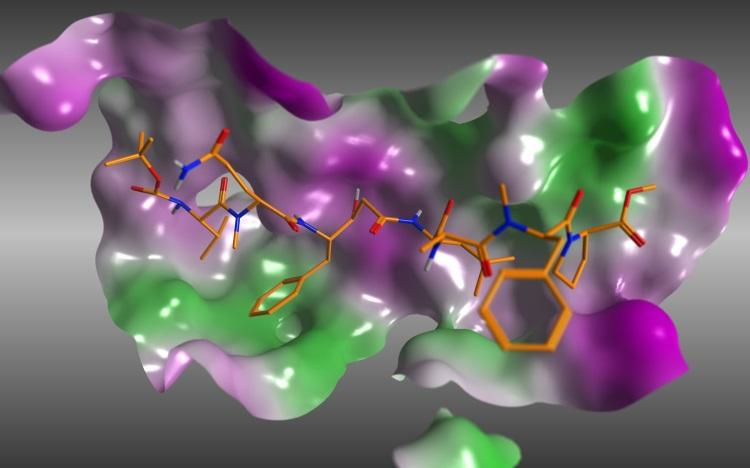
\includegraphics[width=0.9\textwidth]{Images/bace_scheme1.jpg}
  \end{subfigure}
  \begin{subfigure}
  \centering
  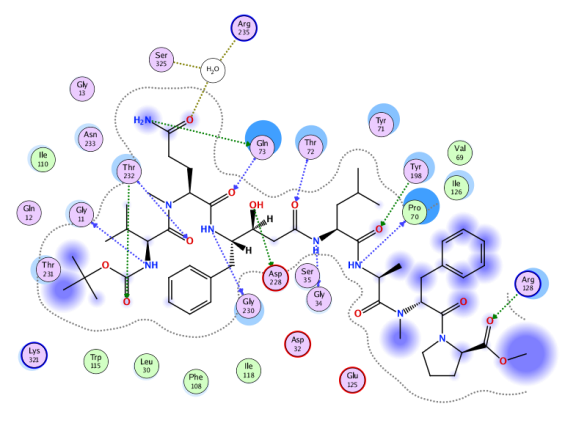
\includegraphics[width=0.9\textwidth]{Images/bace_scheme1B.png}
  \end{subfigure}
  \caption{Scheme 1.  Depiction of BACE-1 binding site (top) using the ligand from PDB code 3UQP along with the protein-ligand interaction (bottom)}
  \label{fig:bace_scheme1}
\end{figure}


Although scientific rigor alongside computational and experimental interplay can enable a much deeper understanding of the key factors influencing binding, they are more often restricted to the specific chemical series that was used for interrogation in the binding affinity optimization cycle.  It is seldom that such learning can be extended widely and hence provides limited value to the broader scientific community.  To circumvent such limitations and expand the scope to address several BACE-1 inhibitor chemical and structural classes, multiple LBD approaches were pursued to identify the sweet spot between computational rigor and trade-off for meaningful compromise that would allow rapid and routine evaluation of new compound ideas in the day-to-day iterative lead optimization cycle.  

\subsection{Methods}

The current dataset includes 1,547 synthetic human BACE-1 inhibitors reported in scientific literature over the past decade with protein…ligand x-ray structures available for over 250 of them in the PDB \cite{rose2010rcsb}.  Experimental IC50’s are also reported for 1,486 compounds and Kd/Ki reported for another 43.  The dataset covers compounds originating from at least 30 different laboratories that include academia, biotechnology, and pharmaceutical companies and spans across the globe in terms of their origin, cautioning on the inhomogeneity of experimental observation \cite{kramer2016comprehensive} used for statistical modeling.  The structures and reported activities for all the compounds were retrieved from either ChEMBL \cite{gaulton2011chembl} or from the original source publication using the citation information from PDB.  In assembling the ligand dataset, only publications that reported a solved x-ray ligand…BACE-1 structure was considered as this provides a reasonable premise to guess on the potential binding mode (bioactive conformation) of the closely related medicinal chemistry derived analogs reported in the same article as part of the structure-activity relationship (SAR).  We have made the ligand dataset publicly available in a convenient CSV format \cite{wu2017moleculenet}.

The physicochemical attributes for the 1547 ligand dataset were computed using BIOVIA’s Pipeline Pilot \cite{systemes2016biovia} and vary between 138 to 1350 for molecular weight (MW); -6.6 to 7.4 for logD; -5.1 to 7.6 for AlogP; 16 to 525 for polar surface area (PSA); 0 to 18 for H-bond acceptor (HBA); 1 to 15 for H-bond donor (HBD); 0 to 40 rotatable bonds; 10 to 90 for heavy atom counts for the reported experimental pIC50’s ranging from 2.5 to 9.5.  As would be apparent, the chemistry captures very small synthetic fragments and large molecular weight oligopeptide and their mimics.  The ligand efficiency (LE) varies between 0.2 to 0.5, binding efficiency index (BEI) ranges from 8 to 22, and the surface efficiency index (SEI) mostly between 4 and 12 \cite{abad2010ligand}.  A distribution of the various physicochemical property profiles (Supporting information S2) reveal that the dataset attributes is not skewed and spans the individual space with a Gaussian spread.  
The global 3D alignment of all the analogs from multiple chemical scaffolds was achieved by following the steps outlined in Figure \ref{fig:bace_scheme2}.  Chain A of 2QP8 (PDB code) was used as the reference, as this structure had one of the best available resolutions (1.5Å) reported when this work was initiated.  Each of the reported PDB structures for the BACE-1…inhibitor x-ray complex was structurally aligned to the above reference using the structalign script available within the Schrödinger’s MAESTRO \cite{maestrorelease20142} suite of programs.  The protein, metal ions, and solvent were subsequently removed from the aligned structures and only one ligand structure from each PDB entry was retained for further processing.  The structure data file built based on protein superposition (containing all the aligned ligands) was uploaded to the molecular database spreadsheet within MOE \cite{moeversion2012chemical} from Chemical Computing Group.  The ligands were subsequently cleaned (bond orders fixed) and prepared by the addition of hydrogens and molecular charges as deemed appropriate.  This procedure now provides an alignment of the diverse ligands in a universal chemical space as would be seen by the protein target.  It also minimizes the pharmacophore and shape bias elicited by the molecular superposition algorithms, and underpins the notion that structurally similar ligands need not bind in a similar way. \cite{subramanian2012integrated}

\begin{figure}
  \centering
  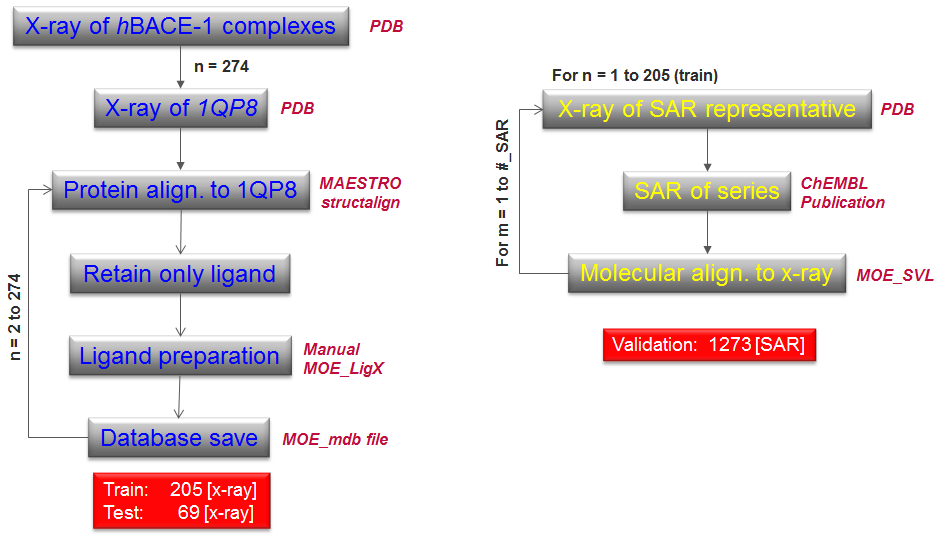
\includegraphics[width=0.9\textwidth]{Images/bace_scheme2.png}
  \caption{Scheme 2. Workflow for the Training, Test, and Validation Set Compound Alignment Used for 3D-Field Based Approaches.}
  \label{fig:bace_scheme2}
\end{figure}

The 274 compounds assembled in this manner (x-ray of aligned hBACE-1…ligand complex) formed the basis of the training (205) and test (69) sets respectively and were used for the 3D molecular alignment dependent approaches pursued in this study.  Since the bioactive conformation for each ligand is now identified (based on the x-ray complex), all medicinal chemistry derived structural analogs within each scaffold reported as part of the SAR exploration in the respective publication were aligned to each individual reference x-ray structures (Figure \ref{fig:bace_scheme2}, right) to yield the final 1,273 validation set analogs that did not have an experimental x-ray structure disclosed in public literature.  No similarity cutoff threshold was used for the SAR compounds since these were standard R-group analogs belonging to the same chemotype that is represented by the x-ray structure reported in the same publication.

The alignment protocol follows the procedure described earlier in literature. \cite{subramanian2012integrated}  Specifically, the ligand coordinates extracted from the BACE-1 complex x-ray structure reported in each individual publication was used as the reference frame (Figure \ref{fig:bace_scheme2}, right) and the SAR analogs reported in that publication were superposed to the chosen reference using the fragment\_superpose and flexalign\_manual svl scripts available from MOE.  Further refinement was achieved through subtle constrained minimization of each of the aligned ligand to achieve maximum overlay with the reference structure per the refine option implemented within the flexalign\_manual.svl script.  This procedure of choosing the individual x-ray reference and SAR analogs was iterated for each publication (see S1 supporting information) and the consolidated alignment of all the reference compounds (now part of the training set) and the SAR analogs (now part of the validation set) comprise the full dataset used for the modeling exercise. 

An additional 69 ligand bound x-ray structures were grouped as the prospective test set since these complexes do not have reported IC50 values, but some of them have either Ki/Kd disclosed instead.  The predicted binding affinities would then offer a decent starting point if scaffold hopping exercise need to be pursued for any of these chemical series.   Succinctly, the published x-ray of BACE-1…ligand complex constituted the source of the 205 training set compounds and the reported SAR in scientific literature formed the basis of the 1273 validation set molecules such that the latter has at least one close representative in the training set. 
In order to ascertain if such strenuous computational rigor described above is required to obtain statistically meaningful and robust predictive QSAR models, additional LBD approaches were also pursued.  These include the standard QSAR approaches that use the traditional binary fingerprints or molecular descriptors as computed by Canvas \cite{canvasrelease20131} from Schrödinger.  For instance, the 1000 most informative bits from linear, radial, dendritic, and MolPrint2D fingerprints \cite{sastry2010large,an2013kernel}, were used to develop qualitative classification models while the constitutional, physicochemical and topological descriptors computed using Canvas were used to build quantitative regression models.  Both the qualitative and quantitative models included linear, non-linear, and deep learning techniques \cite{ramsundar2015massively}.  Such a thorough coverage of the interdependence of dataset, descriptor, and statistical approach for one protein target represented by diverse chemical scaffolds should provide standard baselines when approaching similar problems in a lead identification or optimization cycle within a preclinical drug discovery setting.

\subsection{Results}

\subsubsection{Chemistry Space}
Prior to analyzing the outcomes from the different approaches and models, it is pertinent to chart out the chemical space occupied by the training and validation set BACE-1 inhibitors as this would provide some granularity for the well-recognized model applicability domain concerns \cite{sheridan2015relative}.  Since the model generation involved multiple descriptor features, the chemical space was generated using the same feature space.  The first three principal components (PC) were computed using extended connectivity fingerprint (ECFP6) \cite{rogers2010extended}, Canvas constitutional, physicochemical, and topological descriptors \cite{sastry2010large}, as well as Bemis-Murcko Tier-1 (topography with atomtype annotation) or Tier-2 (topography) molecular framework scheme \cite{bemis1996properties}.  Figure \ref{fig:bace_1} depicts the scatter plot of the PC1 and PC2 space derived from some of the procedures mentioned above.  As would be expected, the Tier-2 reflects the minimal diversity points in the compound space since this represents the 2-dimensional (2D) shape and geographical topology of the varying chemotypes considered in this study.  The 2D skeleton terrain sheds light on the chemical framework heterogeneity (Figure \ref{fig:bace_1A}) within a dimensionality reduction visualization context, with the expected homogenous distribution (overlap) for the validation set around the training set compounds.  An alternate perspective obtained using the radial ECFP6 fingerprints captures the subtle and varied contours and represents a few clusters (Figure \ref{fig:bace_1B}).  A pairwise comparison of the training set compounds using ECFP6 fingerprint and Tanimoto similarity computed via Canvas is provided in supporting information S3.  The macroscopic chemistry space view obtained by computing the various constitutional, physicochemical, and topological properties together reflect on the broad property based diversity of the inhibitors considered.  The scatter distribution, being continuous and not overly islandic, also provides enough motivation to have confidence in the models being developed.  The plots also highlight that the positioning of the validation set in comparison to the training set compounds is not unreasonable to raise concerns in the predictive capability (model applicability domain) of the models being developed using either the fingerprint or descriptor space (Figure \ref{fig:bace_1C}).

\begin{figure}
\centering
\begin{subfigure}
  \centering
  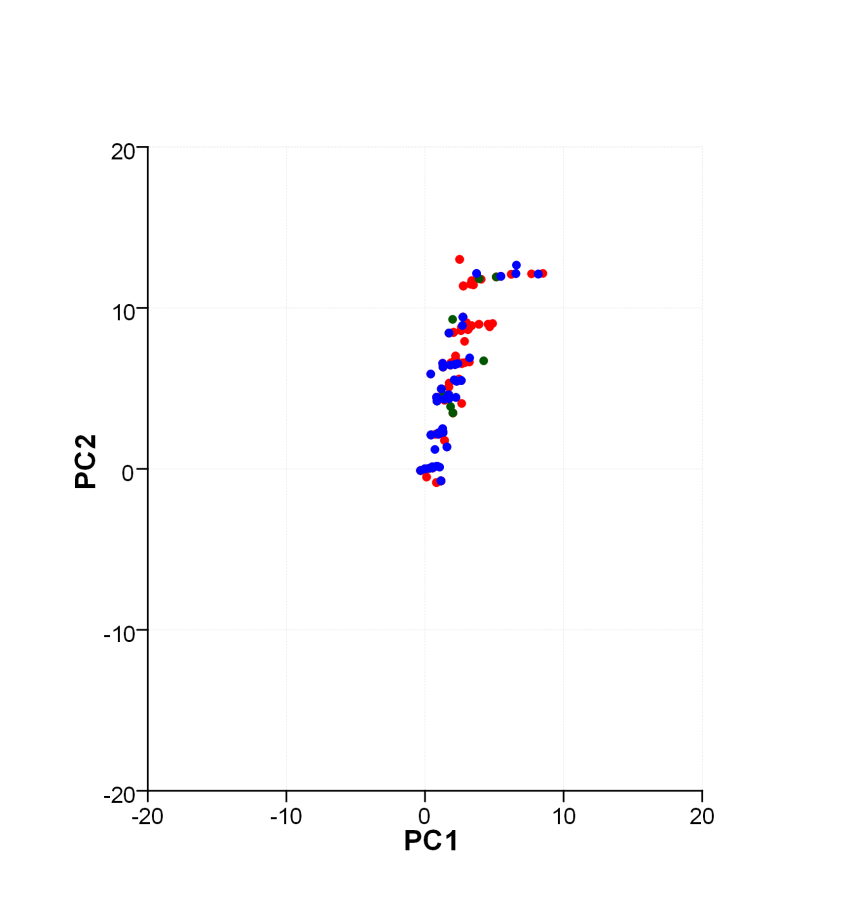
\includegraphics[width=0.3\textwidth]{Images/bace_figA.png}
  \caption{A)  Tier 2 Bemis-Murcko framework}
  \label{fig:bace_1A}
\end{subfigure}
\begin{subfigure}
  \centering
  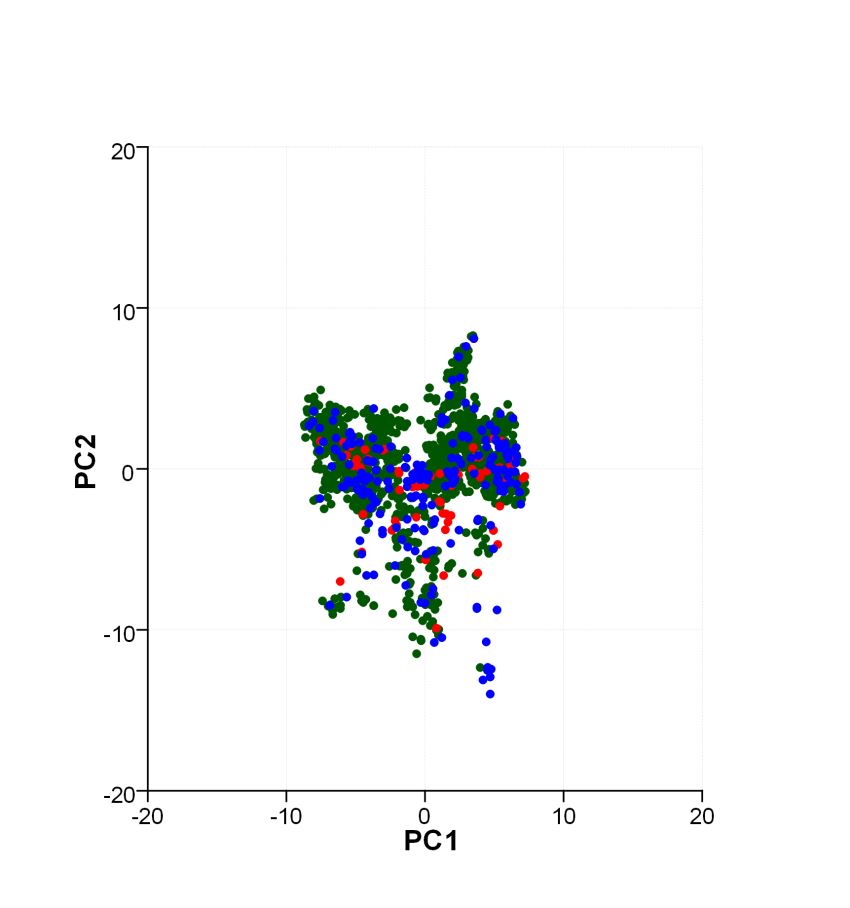
\includegraphics[width=0.3\textwidth]{Images/bace_figB.png}
  \caption{B) ECFP6 fingerprints}
  \label{fig:bace_1B}
\end{subfigure}
\begin{subfigure}
  \centering
  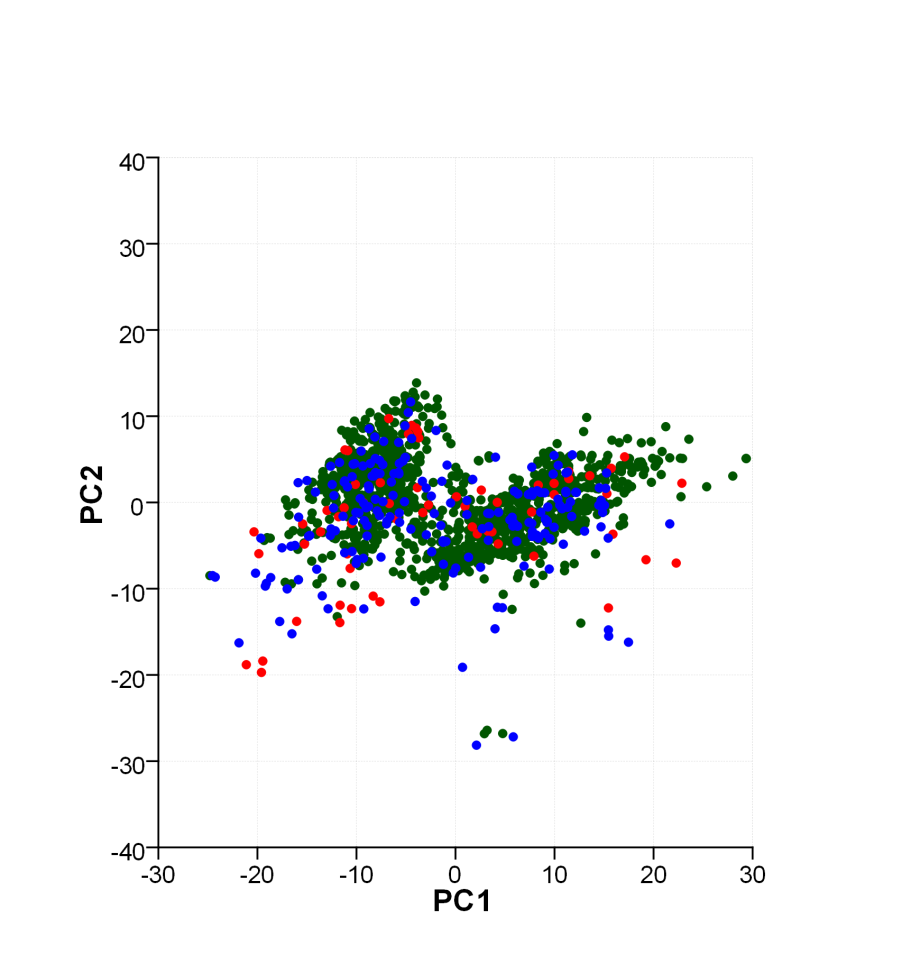
\includegraphics[width=0.3\textwidth]{Images/bace_figC.png}
  \caption{C) Canvas descriptors}
  \label{fig:bace_1C}
\end{subfigure}
\begin{subfigure}
  \centering
  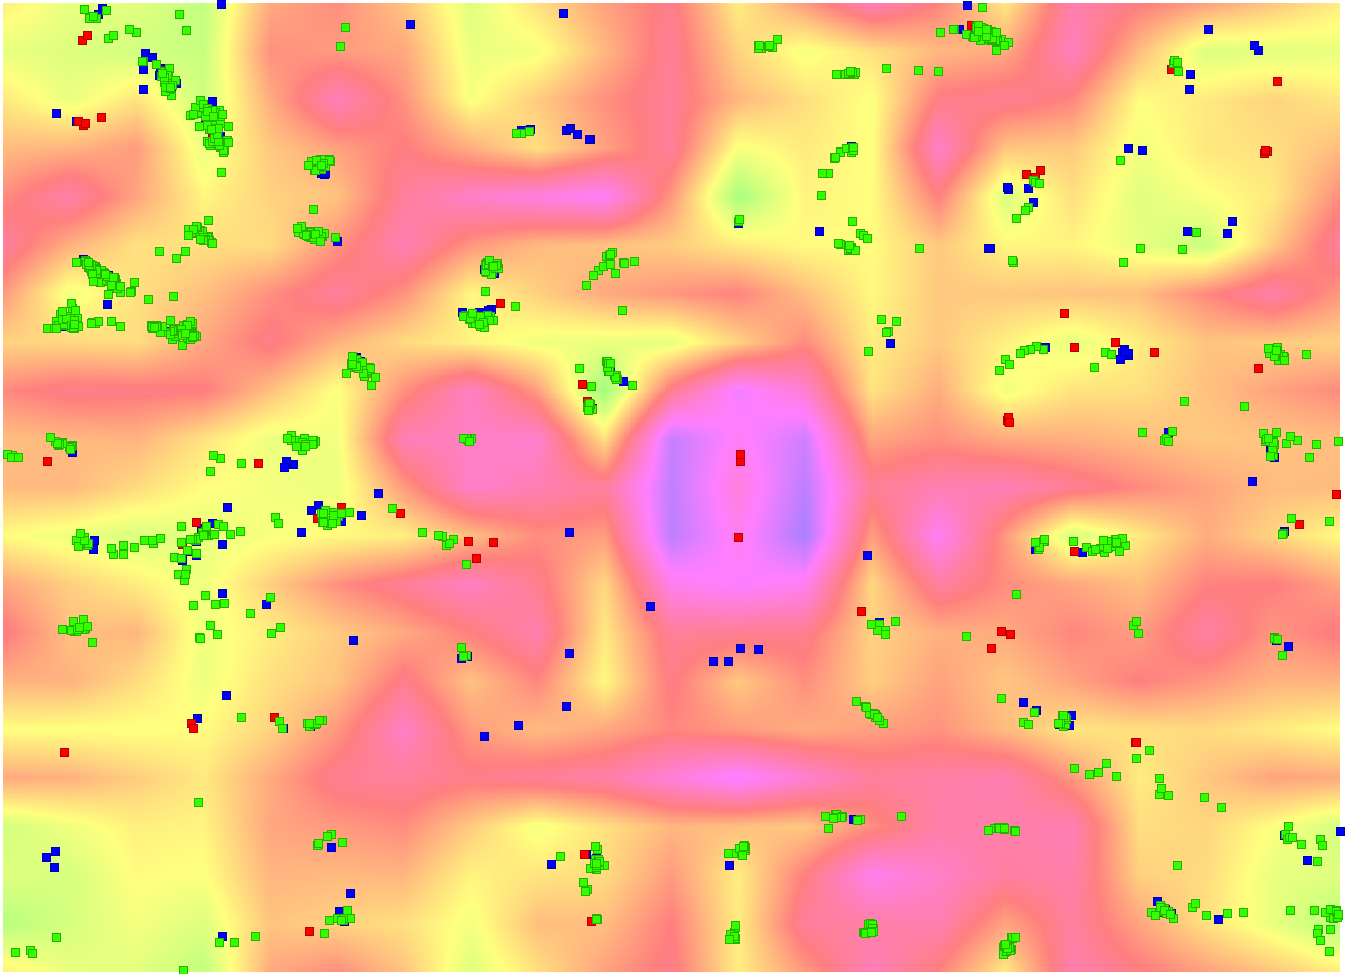
\includegraphics[width=0.3\textwidth]{Images/bace_fig1D.png}
  \caption{ D) Scaffold grouping on a SOM for the training (blue), validation (green), and test (red) set compounds.}
  \label{fig:bace_1D}
\end{subfigure}
\caption{PCA plot for the 1547 BACE-1 inhibitors.  Training, validation, and test set compounds colored in blue, green and red respectively.}
\label{fig:bace_1}
\end{figure}

Two dimensional self-organizing map (SOM) \cite{kohonen1998self} is another dimensionality reduction technique that provides an orthogonal viewpoint compared to the previous approaches \cite{osolodkin2015progress}. The outcome from SOM using the Canvas descriptors is shown in Fig. 1d.  It should be noted that the SOM implementation in DataWarrior \cite{sander2015datawarrior}, uses Rubberbanding forcefield approach that translates the similarity better than the traditional PCA.  Since the SOM clustering is based on similar compound pairs and neighborhood relations, the diversity of the chemical scaffolds considered in this study is reminiscent in the distinction shown between the topological neighbors and close neighbors.  The SOM depiction in Fig. 1d also shows that majority of the training and validation set compounds have clear topographical neighbors, while the training and test set compounds offer additional close neighbors that can potentially be exploited for SAR exploration, if needed. 

\subsubsection{Biological Property Landscape}

Although the unsupervised approaches for modeling the chemical space present a clean picture of confidence for pursuing modeling activities, additional evaluations were undertaken on the dataset to delineate potential disconnects in the biological property space being modeled when relatively minimal changes are incorporated to the structure.  The SkeletonSphere descriptor scheme implemented in DataWarrior \cite{sander2015datawarrior} was used for the chemical descriptions of the training and validation datasets. The structure activity landscape index (SALI) \cite{guha2008structure} that provides a disconnect measure between the biological observation ($\Delta \text{pIC50}$) and the extent of chemical diversity (1 – similarity) for each compound pair was subsequently computed and incorporated within Figure \ref{fig:bace_2A} of the affinity (pIC50) scatter plot for each of the molecule pair being compared.  Approximately 2,765 pairs were identified using a similarity cut-off threshold of 95\% (Supporting information S4).  Among these, only 51 pairs can be attributed solely to the training set and this provides another inference for the compound diversity within the training dataset.  Among the 2,714 chemical similarity pairs within the validation set, activity cliffs $\geq 2$ log units are exhibited by at least 102 pairs representing ~4\% of the validation set.  These experimental observations suggest instances where subtle changes to structure has profound impact on the IC50 being measured in spite of the conserved modifications to the structure.  While such biological property space ruggedness cautions on the predictive capabilities of the in silico models being developed, it should be emphasized that the overall terrain is pretty smooth with ~2,200 pairs exhibiting $\Delta \text{pIC50} < 1$ log unit.  Irrespective of the model performance on the molecules that demonstrate activity cliffs, the experimental observations shed light on the expected microenvironment (steric, electrostatic, H-bond, etc.) hotspots that need to be paid attention to, besides the black box modeling outcome.  


Figure \ref{fig:bace_2B} provides a visual depiction of the relationship between the observed experimental affinities with respect to the similarities in the chemical space computed using SkelSpheres descriptors implemented in DataWarrior \cite{sander2015datawarrior}.  The key observation is the finding that training set compounds (blue squares) are spread across the validation set compounds, although not being blown out extensively.  The near neighbors in the validation set that surrounds the training set based on similarity and the SALI index (square size) shows that the biological environment is also smooth to a major extent albeit the anticipated cliffs observed in some instances within the clustered compounds.  
Thus, the analysis of the chemical and biological space reveals that the dataset and modeling space [fingerprints/descriptors] should result in productive and predictive models that could guide affinity optimization efforts for hBACE-1 protein target.

\begin{figure}
\centering
\begin{subfigure}
  \centering
  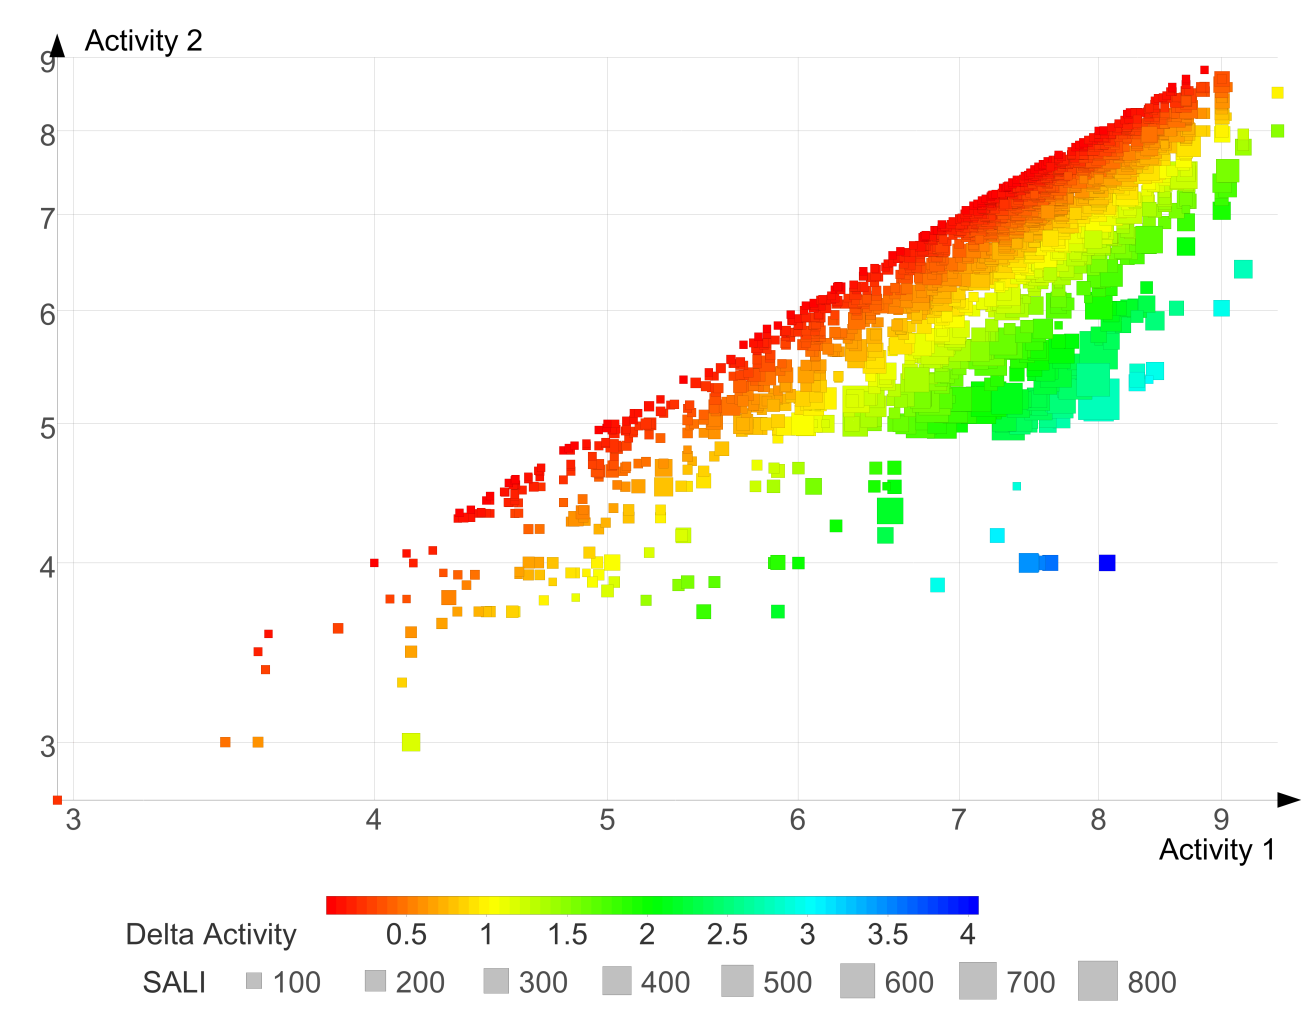
\includegraphics[width=0.9\textwidth]{Images/bace_fig2A.png}
  \caption{a) SALI plot of compound pairs (training and validation) with >95\% similarity.  The x and y axis represent the experimental pIC50 activity values of the compound pairs being plotted (see S4 supporting information).}
  \label{fig:bace_2A}
\end{subfigure}
\begin{subfigure}
  \centering
  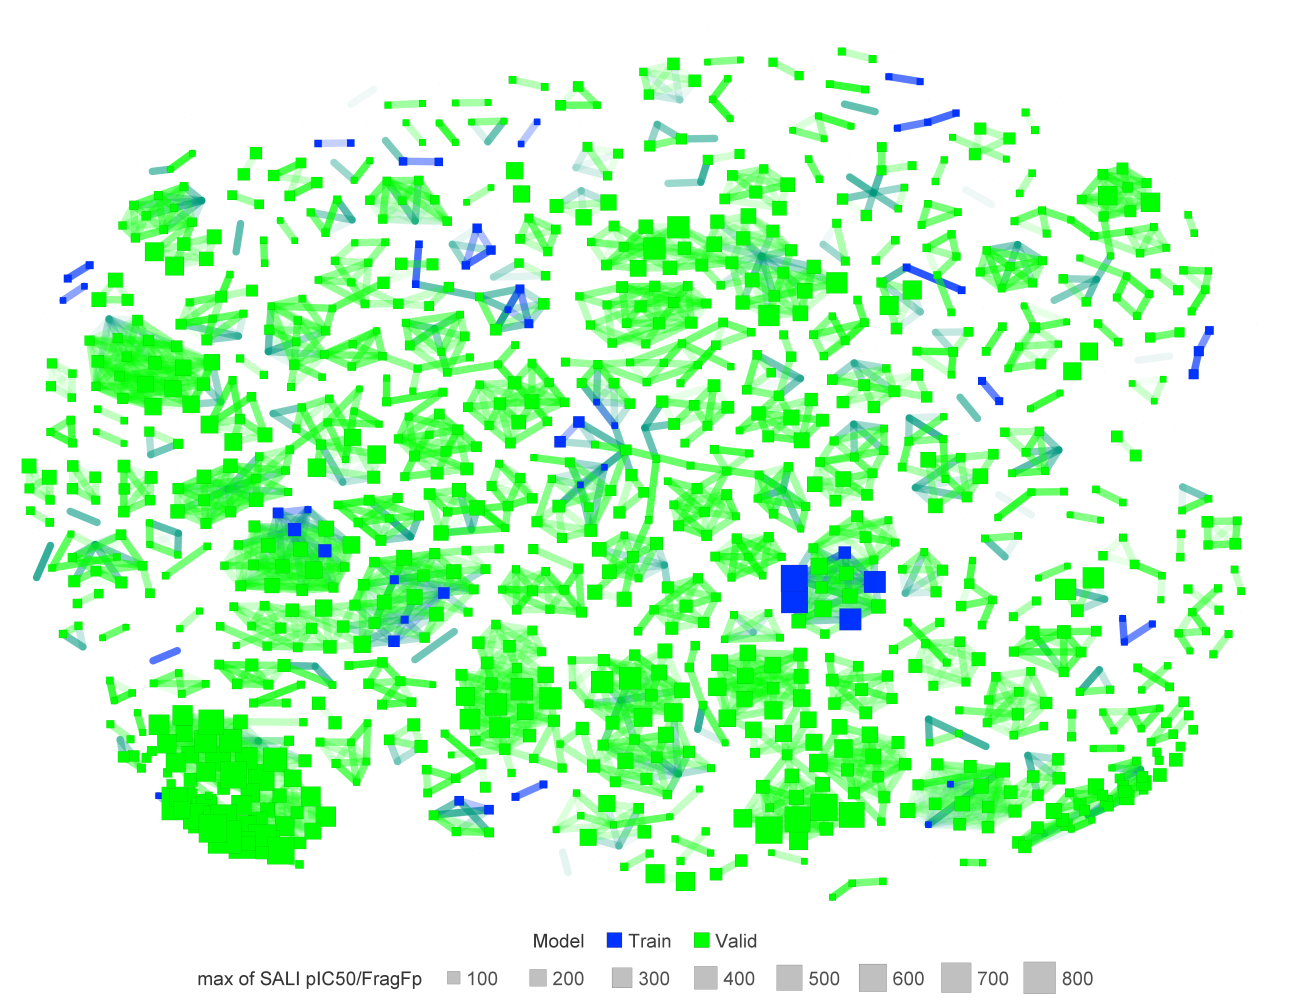
\includegraphics[width=0.9\textwidth]{Images/bace_fig2B.png}
  \caption{b) Activity cliffs (marker size) for the training and validation set grouped based on their neighborhood similarity relationships.}
  \label{fig:bace_2B}
\end{subfigure}
\caption{Plots of compound pairs and activity cliffs.}
\label{fig:bace_2}
\end{figure}

\subsubsection{Classification}

With the confidence provided by the chemistry and biology spaces described above, the modeling domain is expected to perform reasonably well and the same can be gleaned from Table \ref{fig:bace_table1}).  The data set was split into a binary active (IC50 $leq$ 100nM) and inactive class, using a self-imposed cut-off for the experimental IC50.  Apart from the radial fingerprint (ECFP6) described above, fingerprint schemes like the linear, dendritic, and MolPrint2D implemented in Canvas were used to develop additional Bayesian classification models.  These models achieve between 74-93\% classification accuracy on the training set, but only around 55-65\% prediction accuracy on the validation set.  

\begin{figure}
  \centering
  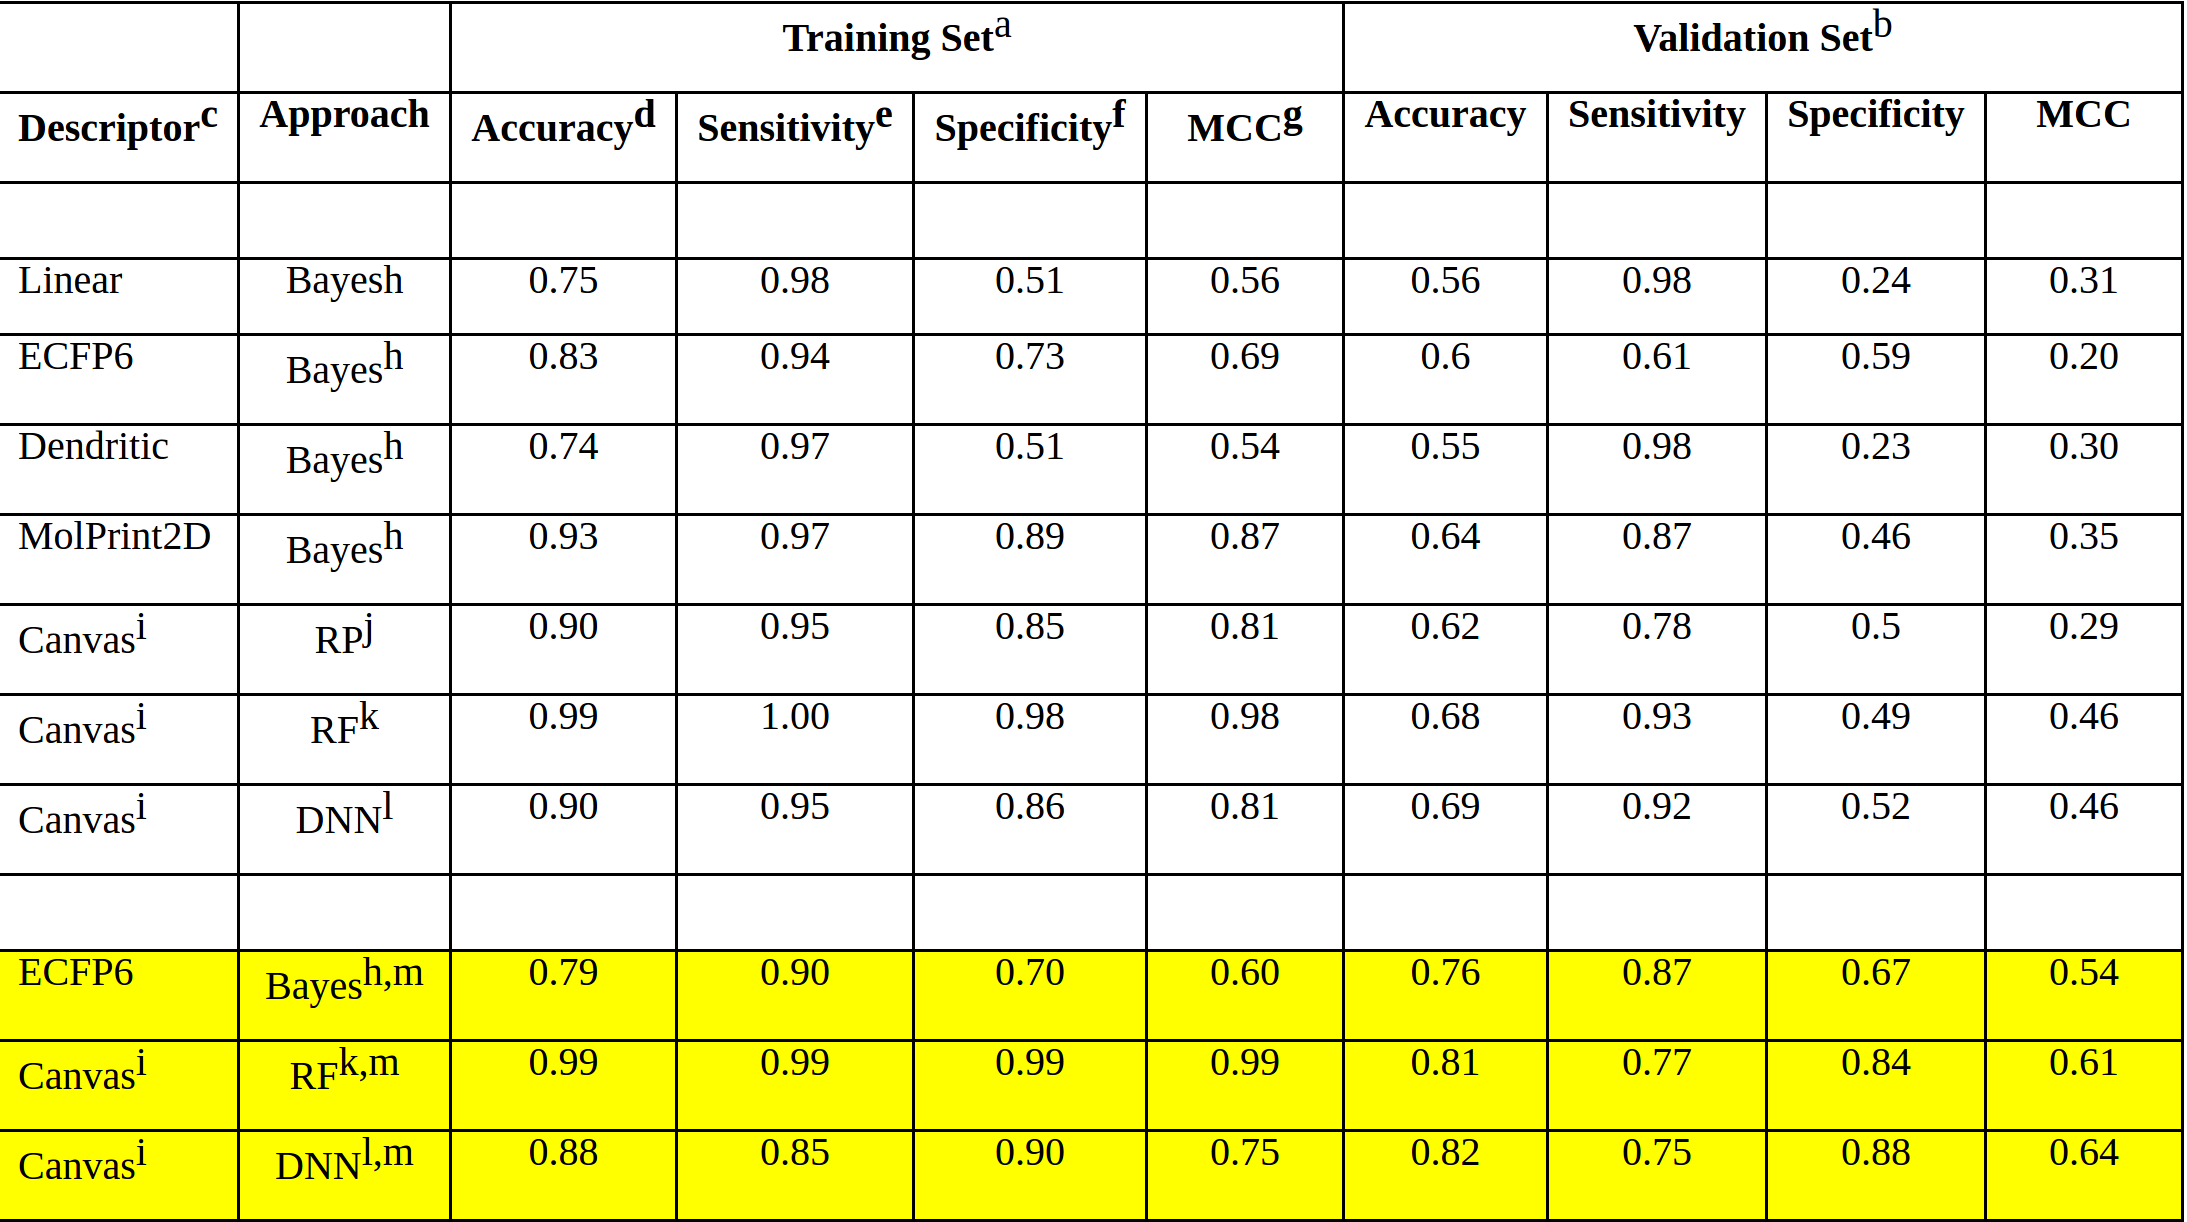
\includegraphics[width=0.9\textwidth]{Images/bace_table_1.png}
  \caption{Table: Statistical Measures for the Various Classification Models Developed in This Work. a) Training Set (205):  Experimentally active (102) with IC50 $\leq$ 100nM; Experimentally inactive (103). b) Validation Set (1273):  Experimentally active (551) with IC50 $\leq$  100nM; Experimentally inactive (722). c) Fingerprint and descriptors as implemented within Canvas modeling suite from Schrӧdinger. d) (TP + TN)/total\_\#\_molecules where TP and TN correspond to true positives and true negatives. e) TP/(TP + FN) where FN correspond to false negatives. f) TN/(TN + FP) where FP correspond to false positives. g) Matthews correlation coefficient. h) Model developed using Bayesian approach as implemented within Canvas modeling suite from Schrӧdinger. i) Constitutional, physicochemical and topological descriptors as implemented within Canvas modeling suite from Schrӧdinger. j) Model developed using recursive partitioning (RP) using Canvas modeling suite from Schrӧdinger. k) Random Forest (RF) model developed using DEEPCHEM package. l) Deep Neural Net (DNN) model developed using DEEPCHEM package. m) Reverse split (yellow fill).  Training Set (1180):  Experimentally active (521) with IC50 $\leq$ 100nM; Experimentally inactive (659); Validation Set (295):  Experimentally active (130) with IC50 $\leq$ 100nM; Experimentally inactive (165).}
  \label{fig:bace_table1}
\end{figure}


In order to construct models with increased predictive power, additional classification models were developed via recursive partitioning (RP), random forest (RF), and DNN statistical techniques using the Canvas constitutional, physicochemical, and topological descriptors.  The RF and DNN models were constructed using the DeepChem library \cite{wu2017moleculenet}. Hyperparameters for RFs and DNNs were selected by model performance on the validation set. The RF models had 10 or 100 trees, and used either square-root, log, and full cutoffs for number of features used when computing tree split. The number of trees and feature-cutoff were selected with grid hyperparameter search on the validation set. The DNN models had a single hidden layer with 1000 units, and dropout .5. Learning rate and decay rate for the DNNs were selected with random hyperparameter search \cite{bergstra2012random}. Both RFs and DNNs demonstrated greater representational power and learned models with classification accuracy in the 90\% range for the training set.  On the validation set, both RF and DNN models achieved stronger predictive power with almost 70\% accuracy, and offered a maximum of 15\% accuracy enrichment compared to the fingerprint based schemes and Bayesian modeling.  The performance of the RP model was comparable to the Bayesian model using MolPrint2D fingerprint scheme (Table \ref{fig:bace_table1}). 

\subsubsection{Regression}

Multiple approaches with increasing sophistication were pursued as part of the quantitative modeling exercise and statistical outcomes are provided in Table \ref{fig:bace_table2}.  At a first glance, the results are underwhelming.  The consistently $ \geq 1$ log unit root mean square (RMS) error for the validation set seem to caution against the application of such approaches within a lead optimization setting in a discovery program.  However, the box plot of the error distribution in Figure \ref{fig:bace_3} reveals that most models performed decently for a majority of the compounds with the exception of some outliers (Supporting information S7).  No single approach outperforms the rest, but CoMFA® seem to have an edge over COMSIA within the SYBYL® application suite and the atom based QSAR modeling (ABM) appears superior compared to the forcefield and Gaussian approximations offered by the MAESTRO suite when 3D-field, -grid based approaches alone are compared.  As expected, MLR that used descriptor feature selection prior to model development performed the worst, but the RF and DNN models built with DeepChem using the Canvas descriptors exhibited comparable performance to the 3D alignment dependent approaches mentioned above (Table \ref{fig:bace_table2}).  The results also highlight that there is only minor prediction enrichment offered by the use of 3D based approaches when compared against 2D descriptor based statistical techniques such as DNNs or RFs, suggesting that LBD with sophisticated statistical techniques recovers many of the advantages of 3D-field based techniques.  The prediction error of the models is reasonable, considering that the experimental observations are drawn from multiple laboratories in various countries.

\begin{figure}
\centering
\begin{subfigure}
\centering
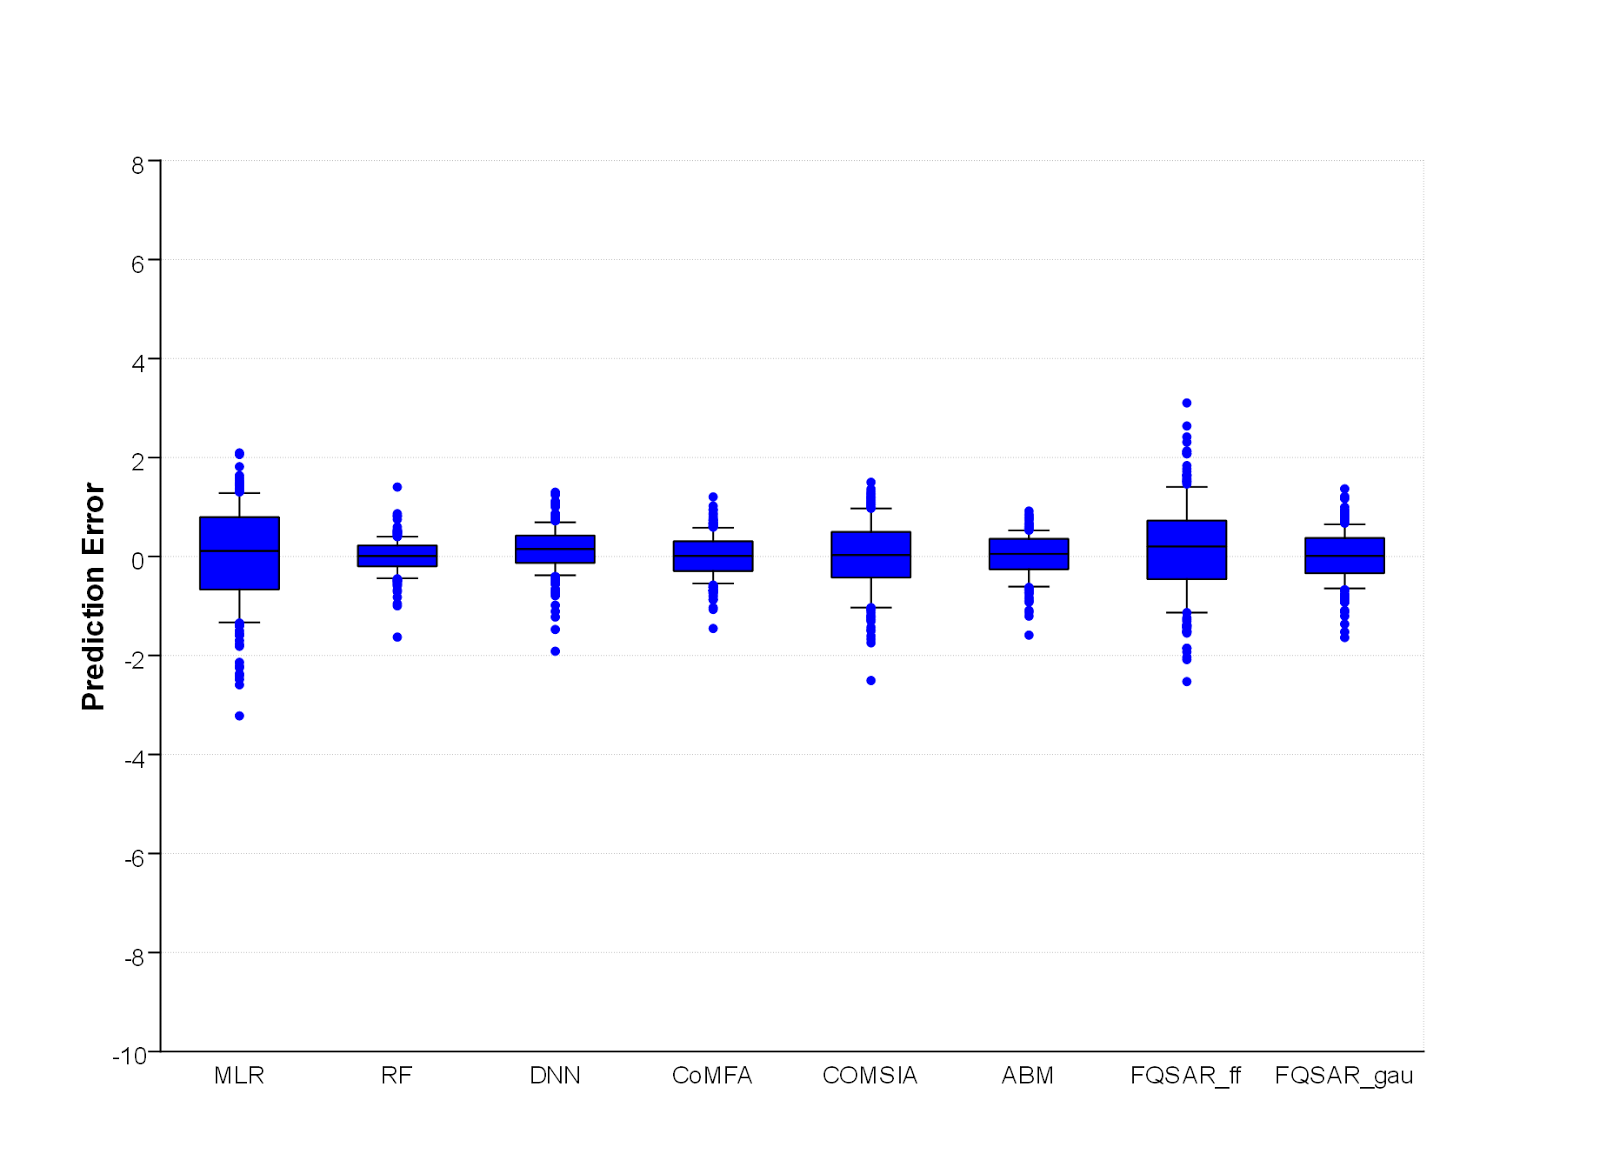
\includegraphics[width=0.9\textwidth]{Images/bace_fig3A.png}
\end{subfigure}
\begin{subfigure}
  \centering
  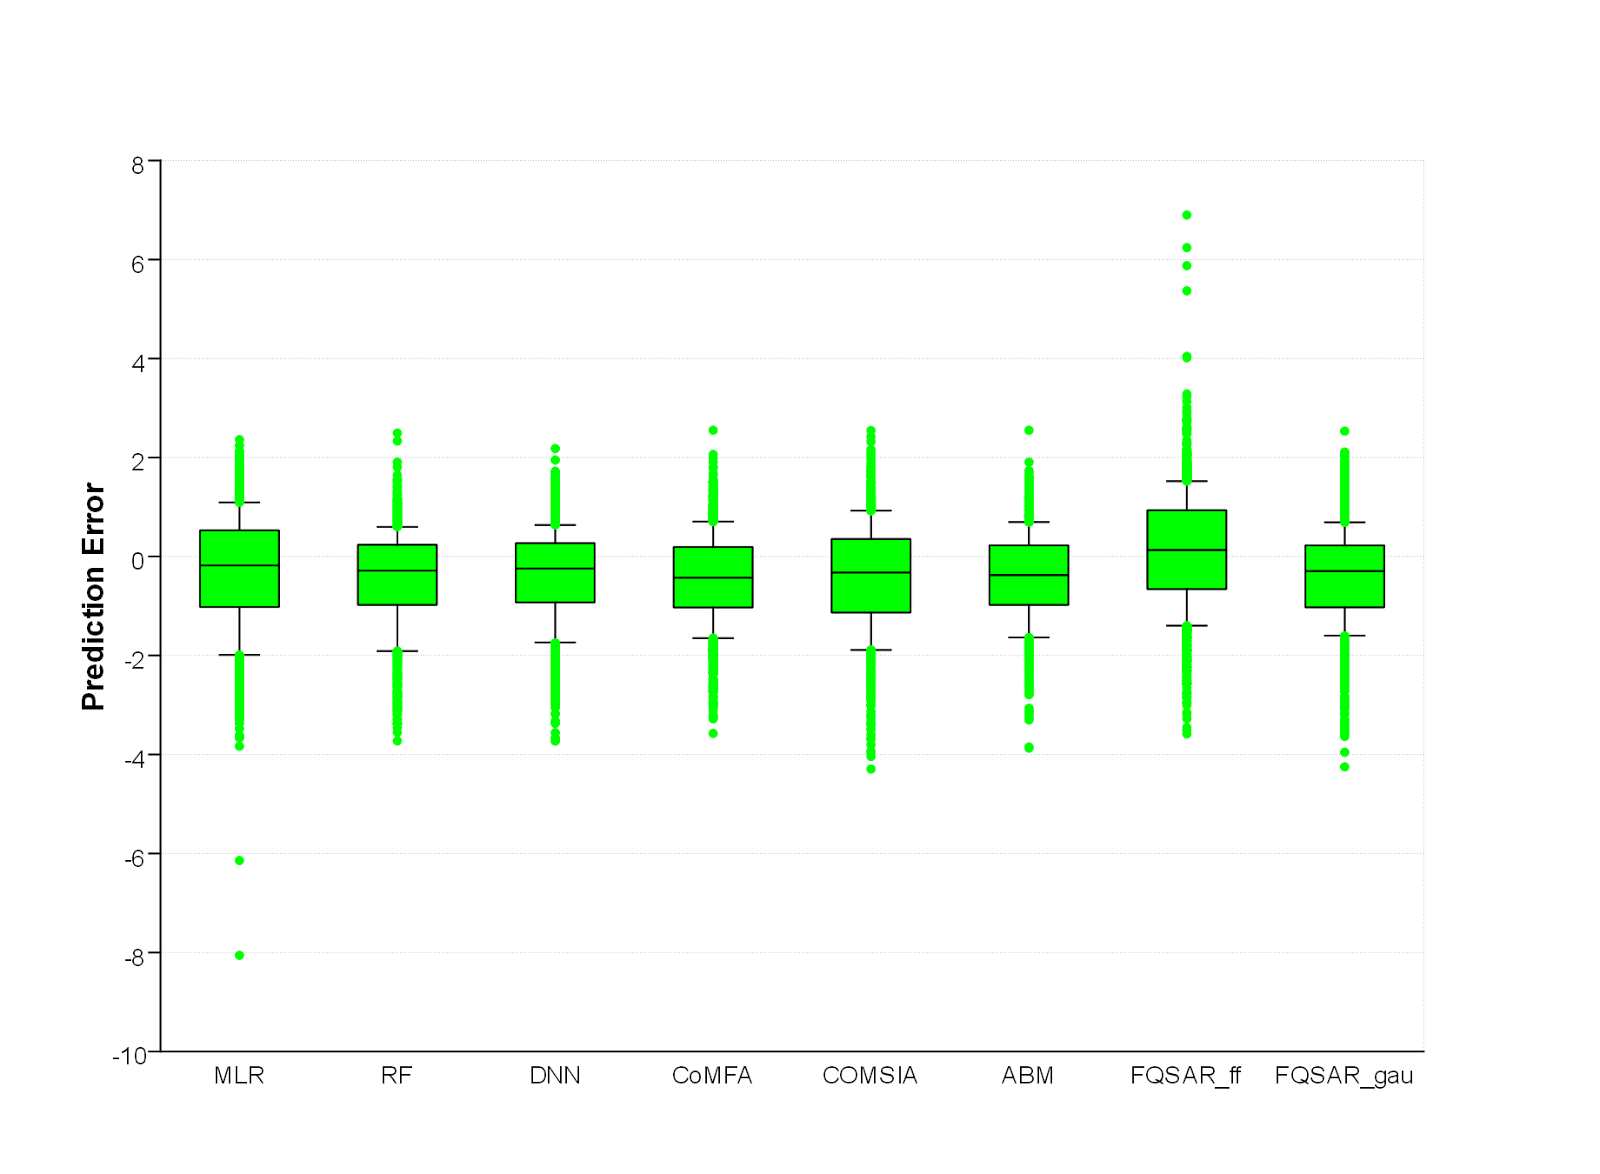
\includegraphics[width=0.9\textwidth]{Images/bace_fig3B.png}
\end{subfigure}
\caption{Box plot of the predicted rms error for the training (blue) and validation (green) set compounds from all the approaches considered}
\label{fig:bace_3}
\end{figure}

\begin{figure}
  \centering
  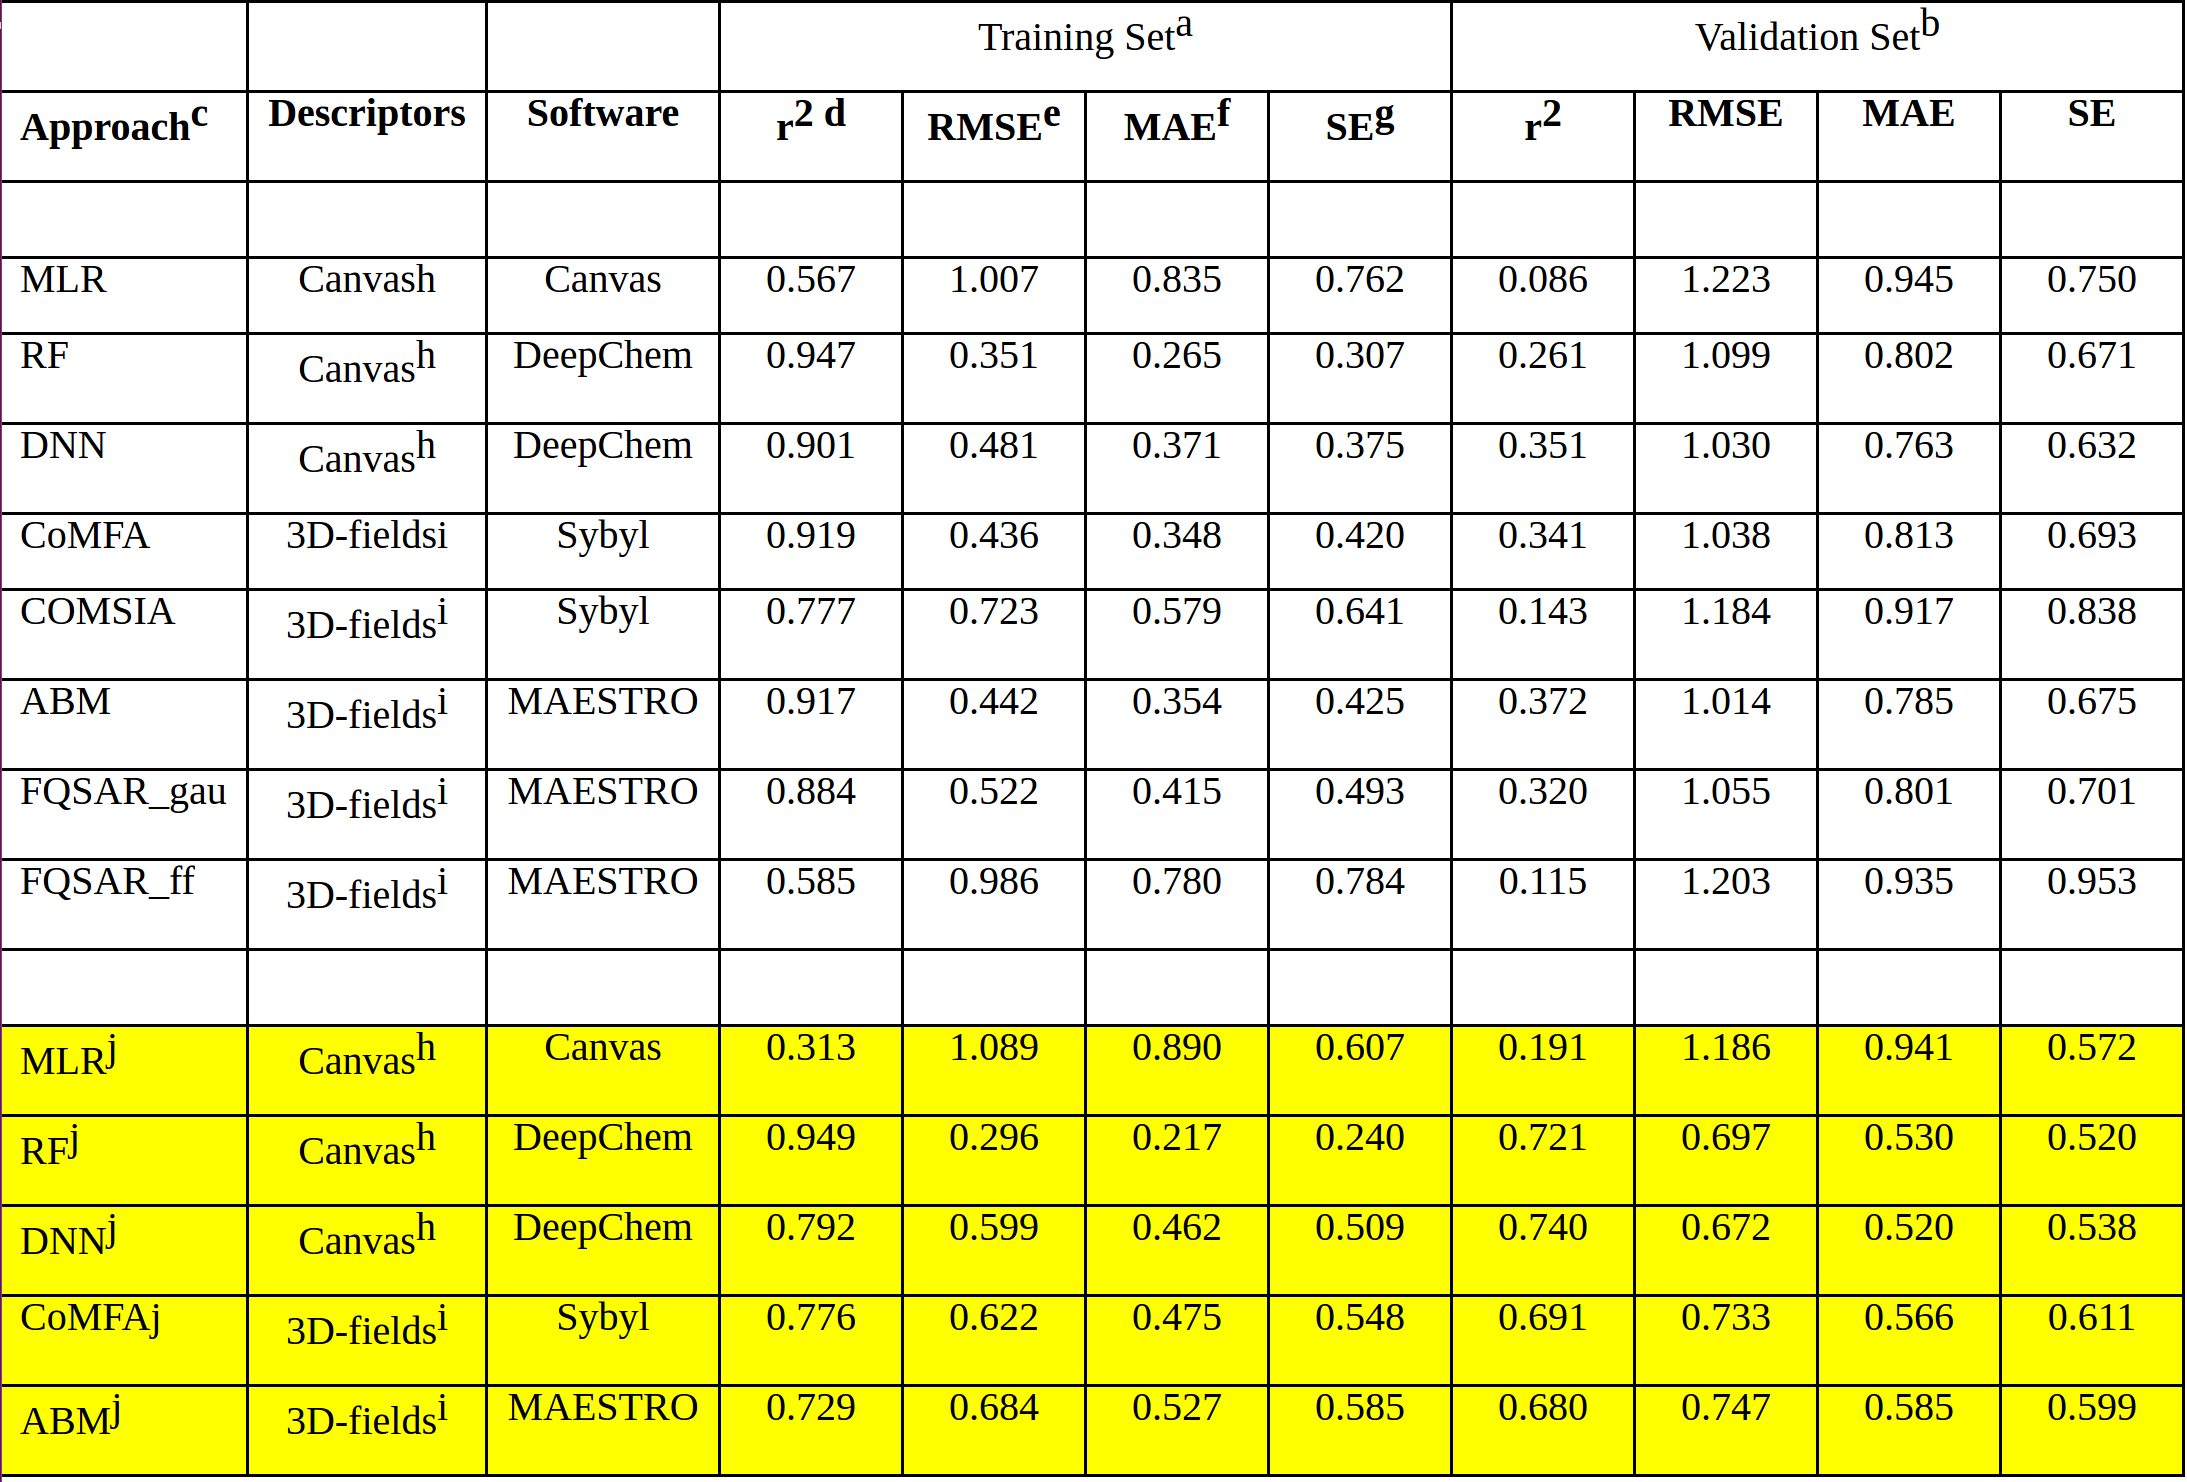
\includegraphics[width=0.9\textwidth]{Images/bace_table_2.png}
  \caption{Table: Statistical parameters for the various quantitative models developed in this work. a) Training Set (205):  Experimentally active (102) with IC50 $\leq$ 100nM; Experimentally inactive (103). b) Validation Set (1273):  Experimentally active (551) with IC50 $\leq$  100nM; Experimentally inactive (722). c) Statistical technique employed (MLR:  Multiple linear regression; RF:  Random forest; DNN: Deep neural nets; CoMFA:  Comparative molecular field analysis; COMSIA:  Comparative molecular similarity index analysis; ABM:  atom-based QSAR model; FQSAR\_ff:  Field QSAR using forcefields; FQSAR\_gau:  Field QSAR using gaussian approximation). d) co-efficient of the fit of a linear regression. e) root mean square error. f) mean absolute error. g) standard error. h) 1D and 2D constitutional, physiochemical and topological descriptors as implemented within Canvas modeling suite from Schrӧdinger. i) 3D-grid based field descriptors utilizing hydrophobic, H-bond donor and acceptor probes as implemented by the individual approaches implemented within Schrӧdinger and Sybyl modeling packages. j) Reverse split (yellow fill).  Training Set (1180):  Experimentally active (521) with IC50 $\leq$ 100nM; Experimentally inactive (659); Validation Set (295):  Experimentally active (130) with IC50 $\leq$ 100nM; Experimentally inactive (165).}
  \label{fig:bace_table2}
\end{figure}

\subsubsection{Reverse Split}

To assess the sensitivity of the various methods on the dataset size, an alternative 80/20 split of the training and validation set was performed by selecting every 5th compound as a validation set member after sorting the full dataset based on the experimental affinity (pIC50).  Such a split would remove any chemotype bias and represent the biological affinity axis uniformly.  This alternate split resulted in 1180 compounds in the training and 295 compounds in the validation set and only methods that performed well for the original dataset was selected (supporting information S10).  As should be expected, the performance accuracy of the selected methods increases, with the machine learning models maintaining a slight edge over their counterparts in classification and regression (Table 1 and 2).  The statistical fit (r2) for the validation set is enhanced dramatically and the RMSE show a 3-fold improvement in error containment compared to the prediction errors for the original 20/80 dataset split, albeit the minor loss in the training set performance (Table 2).  Notably, the machine learning models now slightly outperform the 3D-field based techniques, matching the expectation that learning algorithms grow increasingly powerful with additional data.  The results from the classification models were not dramatic, but did show a tendency of 10-15\% accuracy enrichment for the validation set.  

\subsection{Discussion}

In comparing the relationship between the physicochemical attributes and the experimental affinity for the BACE-1 inhibitors, no distinct patterns emerged as beacons for new affinity improvement designs (Supporting information S2).  For instance, AlogP did not provide clear probabilities between active and inactive compounds since the distribution of actives at the AlogP value around -7 is similar to the ones observed at AlogP values of +7.  There is a near equal frequency of actives and inactives at AlogP values in 1-4 range as well.  Contrary to the lipophilicity trends, the dataset suggests that the minimum molecular weight (MW) should be above 300 for compounds to exhibit IC50 $leq$ 100nM.  However, no discrimination is observed at the higher MW ranges.  The computed ligand BEI \cite{abad2005ligand, abad2007ligand}, reflects the expected inverse correlation as the molecular weight increases and the SEI reveals an exponential decline as the ligand PSA increases imitating on the shallow and exposed binding site occupied by BACE-1 inhibitors (Figure \ref{fig:bace_scheme1}).  The distribution of BEI and SEI histograms [Supporting information S2] also reveal that most of the small molecules are not clustered around their acceptable index values suggesting the suboptimal use of ligand atoms to achieve affinity \cite{mignani2016compound}.  Other features like the H-bond donor or acceptor count also does not guide in setting appropriate filters for affinity improvement activities.  A correlation plot of AlogP vs. PSA advocate a minimal requirement of at least 60Å2 for PSA and an AlogP value $\geq 2$, but is indeed a scatter in distinguishing actives from inactives when viewed from the whole dataset.  Unfortunately, efforts to draw inferences on affinity based on physicochemical parameters (akin to in silico BBB, membrane permeability ADME models) did not yield fruition and this necessitated the development of statistical models reported herein (Figure \ref{fig:bace_scheme3}) to capture the experimental trends with decent predictive power becoming an outcome.

\begin{figure}
  \centering
  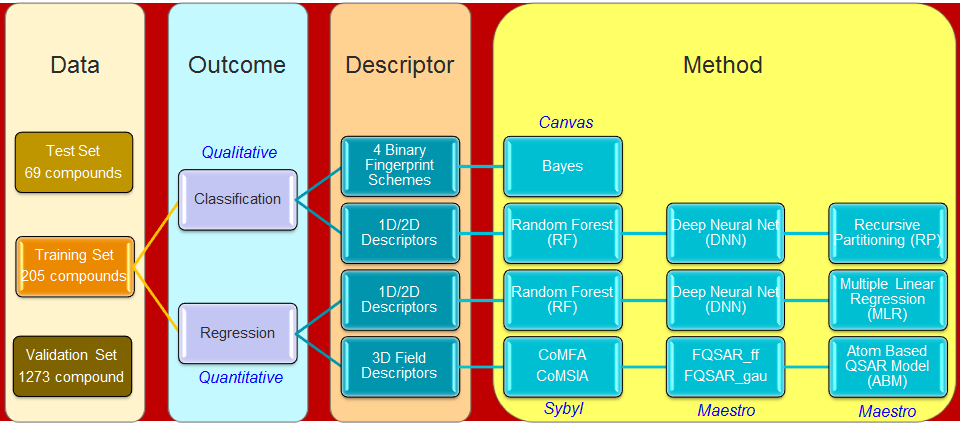
\includegraphics[width=0.9\textwidth]{Images/bace_scheme3.png}
  \caption{Scheme 3.  Modeling scheme and workflow.}
  \label{fig:bace_scheme3}
\end{figure}


Simple Bayesian classification models (Table \ref{fig:bace_table1}) provide a robust framework for filtering ideas, but there is a significant loss in capturing the inactives (specificity) by the use of linear and dendritic fingerprints for the training set compounds.  This loss is evident when the validation set results are inspected and points to a preference for ECFP6 or MolPrint2D among the fingerprint schemes evaluated.  Fortunately, model accuracies could be improved by the use of RF and DNN techniques with more elaborate descriptors.  This enhanced accuracy is likely due to the greater representational capacity of modern machine learning techniques over simpler statistical methods.  At a qualitative level, the modeling outcome for this dataset revealed the capability of machine-learning technique to construct predictive models, given the relatively small 205 training set compounds.This effectiveness for the DNN models is likely due to the use of statistical regularization techniques such as dropout \cite{srivastava2014dropout, mendenhall2016improving}.


The loss in specificity across the different classification models and approaches prompted the consideration of a consensus model to see if aggregating the learning from multiple techniques would improve on the prediction capabilities and minimize the noise.  Table \ref{fig:bace_table3} provides the performance enrichment by selecting 5/7 models (results from linear and dendritic fingerprints ignored).  In examining the results, all the statistical techniques and descriptor schemes seem to learn equally well for the actives, since 95\% and 75\% of the training and validation set is retrieved by at least 4/5 models developed.  However, the classification models still do not seem to have captured all the subtle microenvironment effects from the inactives as the consensus prediction from at least 4/5 models retrieves only ~40\% of the true negatives and is inferior to the predictions from the machine learning methods (Table 1). 


\begin{figure}
  \centering
  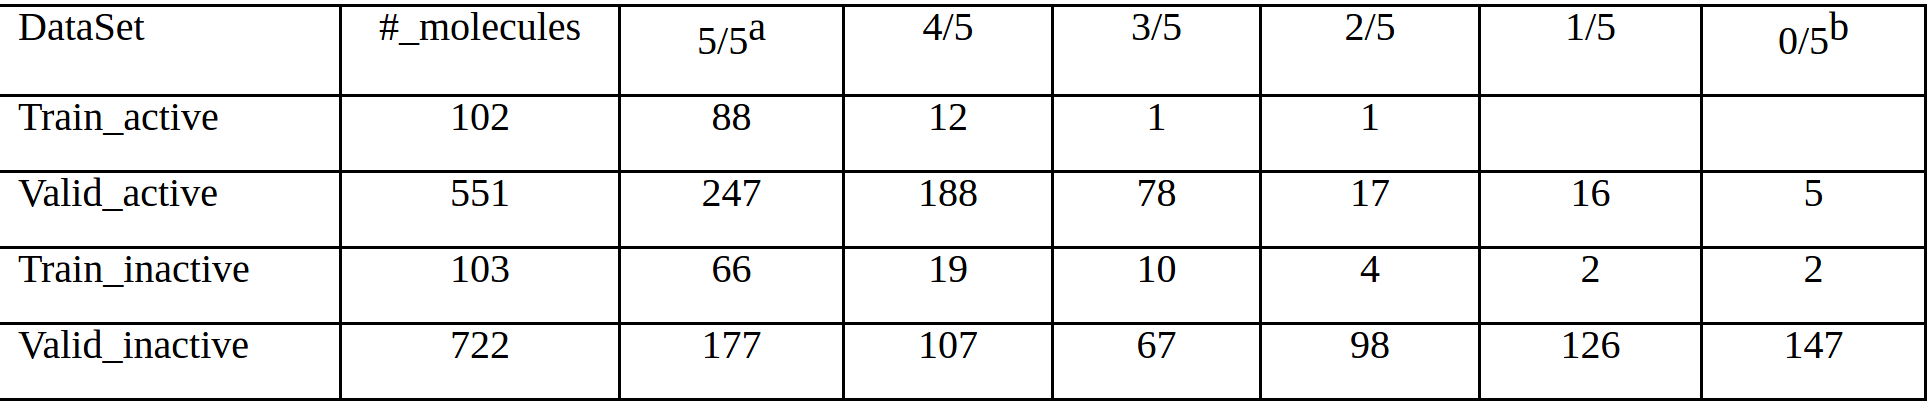
\includegraphics[width=0.9\textwidth]{Images/bace_table_3.png}
  \caption{Table: Performance of the consensus models showcasing classification accuracy enrichment using Bayesian (ECFP6, MolPrint2D), RP, RF, and DNN methods. a) Number of molecules classified correctly by all the 5 models. b) Number of molecules classified incorrectly by all the 5 models.}
  \label{fig:bace_table3}
\end{figure}

Among all the quantitative regression models developed, the outcome from MLR and FQSAR\_ff can be ignored from further consideration (Table \ref{fig:bace_table2}) due to their weakest performance amid the 2D and 3D descriptor based approaches.  Very good correlations between the different approaches provided in Table \ref{fig:bace_table4} (Supporting information S8) clearly vindicate that the dataset is neither sensitive to any specific modeling approach nor is there an advantage for the 3D vs 2D descriptor space used here.  The RF and DNN models are highly correlated (Table \ref{fig:bace_table4}), indicating that both techniques learn similar patterns.  Similarly, the correlation between CoMFA® and FQSAR\_gau suggests the 3D-grid based techniques by both vendors perform comparably, albeit the use of different partial atomic charges schemes.  The pIC50 prediction self-consistency exhibited by the various modeling approaches also encourages re-examination of presumed mispredictions ($\geq 2$ log unit) when compared against the reported experimental observation.  A recent study reported an average 3-fold variability in the observed experimental activity when looking at assay sensitivity over time from a single laboratory \cite{kramer2016comprehensive}.  Hence prediction errors close to 1 log unit (10-fold) should still be treated as fairly reasonable, given the speed and throughput of predictions compared to free energy based methods \cite{wang2015accurate} that strive to achieve predictions within experimental error bars.  Further analysis of the error distribution from RF, CoMFA, and ABM (supporting information S7) suggest that ~40\% of the validation set compounds are predicted with a rms error $\leq 0.5$ log units compared to experimentally determined IC50 values, and another ~30\% when the threshold is moved to 1 log unit.  

\begin{figure}
  \centering
  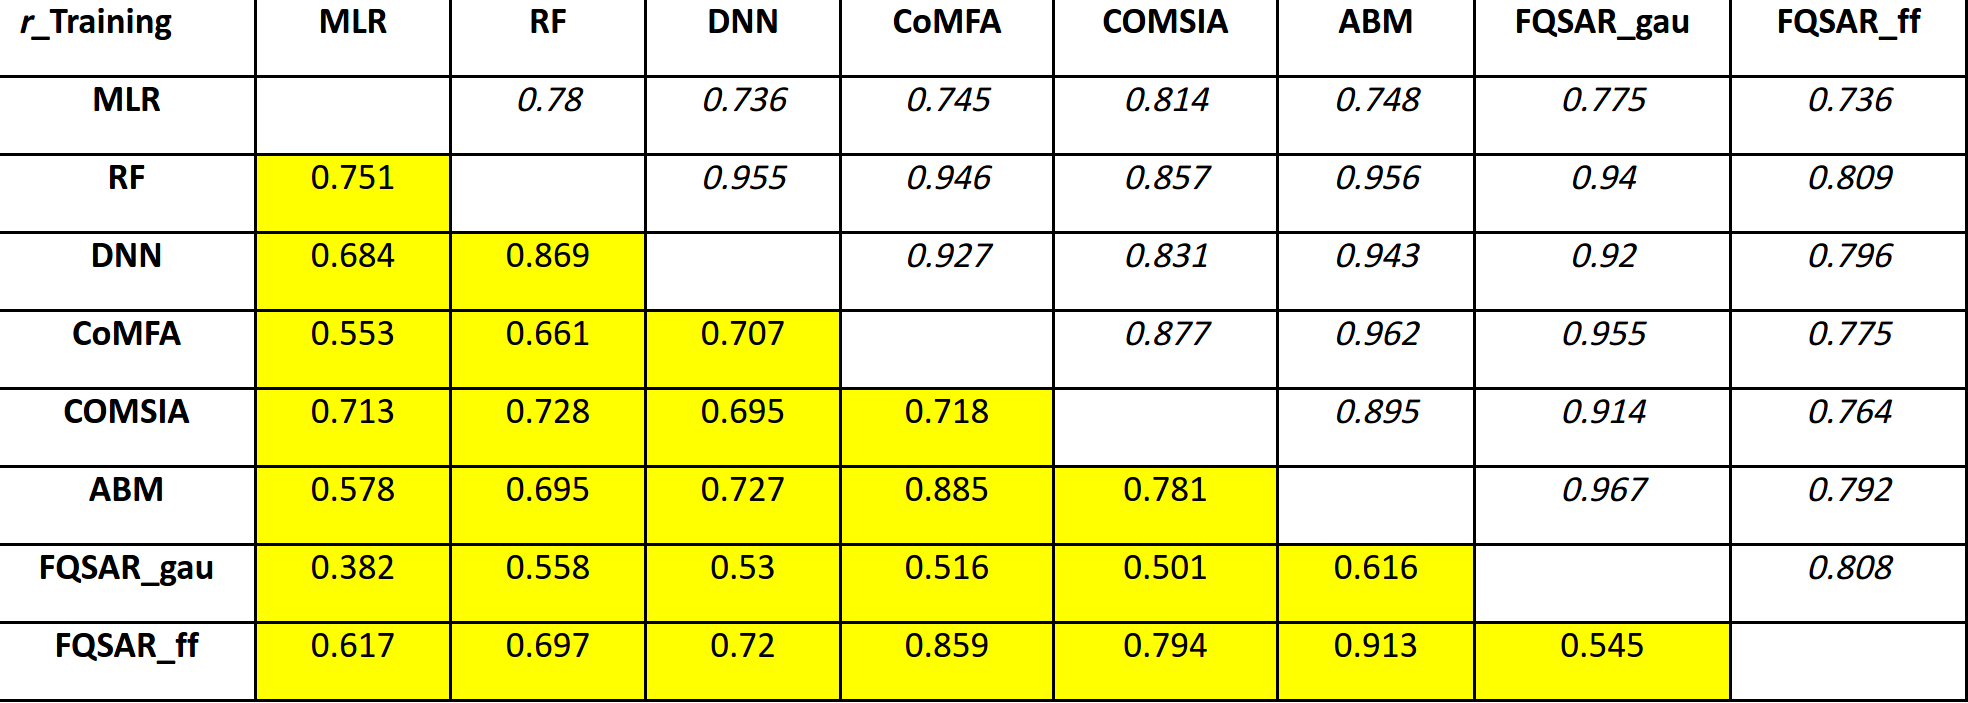
\includegraphics[width=0.9\textwidth]{Images/bace_table_4.png}
  \caption{Table: Correlation matrix for the pIC50 predicted using various approaches for training (top off-diagonal; italics) and validation (bottom off-diagonal; yellow fill) sets.}
  \label{fig:bace_table4}
\end{figure}

Closer inspection of the regression plots from ABM, CoMFA® and DNN shows that the prediction error is relatively high for inactive compounds (Figure \ref{fig:bace_4}).  A reassessment of the errors showed an improvement of 3- to 5-fold for the validation set compounds when only molecules with experimental IC50 $leq$ 1μM are considered (Figure \ref{fig:bace_5}).  Incidentally for this subset, the 2D based RF method outperforms the 3D based techniques and reiterates the fact that reliable models can still be developed using traditional descriptors, but with the use of machine learning methods.  Overall, quantitative modeling of the dataset still offers strong prediction accuracy and can successfully be used in a lead optimization setting. 


\begin{figure}
\centering
\begin{subfigure}
  \centering
  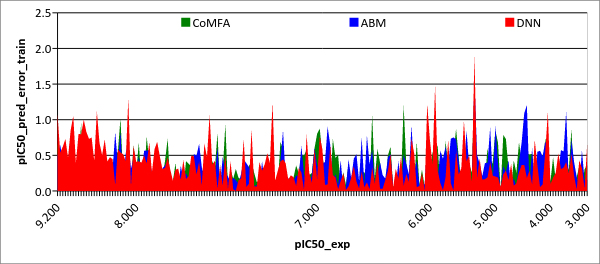
\includegraphics[width=0.9\textwidth]{Images/fig_bace4A.png}
  \label{fig:bace_4A}
\end{subfigure}
\begin{subfigure}
  \centering
  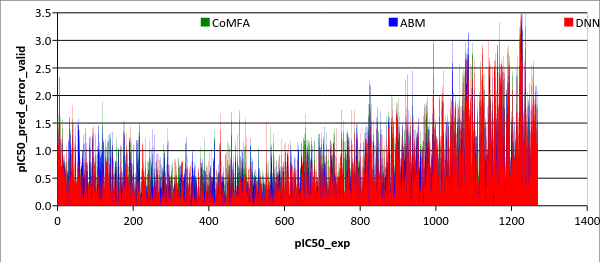
\includegraphics[width=0.9\textwidth]{Images/fig_bace4B.png}
  \label{fig:bace_4B}
\end{subfigure}
\caption{RMSE plot for each of the training (top) and validation set (bottom) compounds based on DNN (red), CoMFA (green) and ABM (blue).  Compounds sorted based on experimental pIC50 values with each vertical line representing the individual molecule’s RMSE with respect to the experimentally observed values.}
\label{fig:bace_4}
\end{figure}

\begin{figure}
\centering
\begin{subfigure}
  \centering
  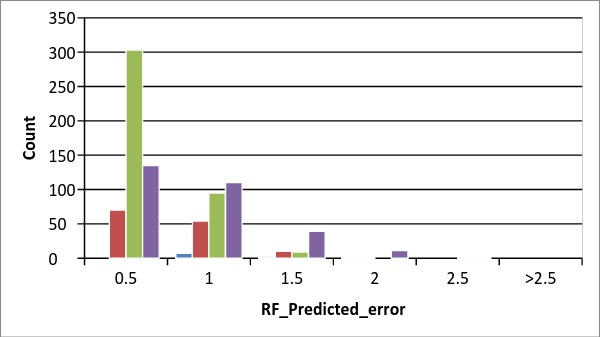
\includegraphics[width=0.9\textwidth]{Images/bace_fig5A.png}
  \label{fig:bace_5A}
\end{subfigure}
\begin{subfigure}
  \centering
  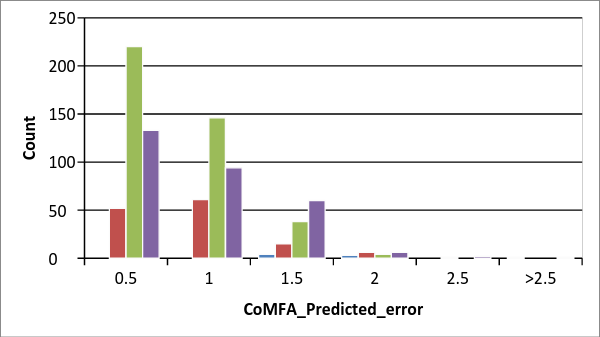
\includegraphics[width=0.9\textwidth]{Images/bace_fig5B.png}
  \label{fig:bace_5B}
\end{subfigure}
\begin{subfigure}
  \centering
  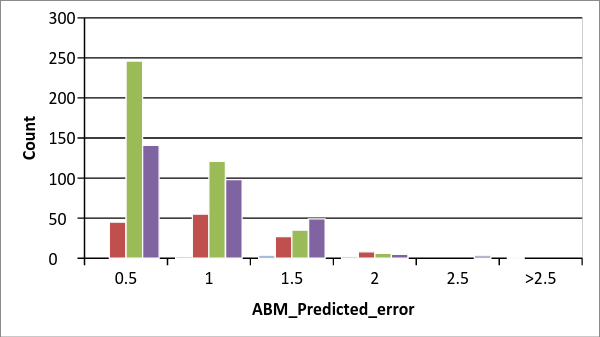
\includegraphics[width=0.9\textwidth]{Images/bace_fig5C.png}
  \label{fig:bace_5C}
\end{subfigure}
\caption{Predicted RMSE distribution spread based on RF, CoMFA, and ABM for the validation compound subset with experimental IC50 $\leq$ 1 microM}
\label{fig:bace_5}
\end{figure}

Redeveloping some of the models using a reverse split of 80/20 training to validation set ratio did result in enhanced statistical fit for the quantitative models and demonstrated a 3-fold improvement in minimizing the prediction errors for the validation set.  Similarly, the classification models were able to achieve accuracy and specificity improvements.  However, the conclusions from the qualitative (Table 1) and quantitative (Table 2) approaches were not game changers to suggest that the dataset size considered here could influence the modeling outcome.  The results support the view that reasonable models with good prediction capabilities can still be developed with a relatively diverse and modest dataset size. This would become more apparent, if parallels can be drawn from the relatively good success of the implemented global in silico ADME models using relatively small datasets \cite{gleeson2011silico, peach2012computational}, as well as the secondary structure prediction based on just the sequence information \cite{kabsch1983good, drozdetskiy2015jpred4}, from a fairly small sample size that stand as a testament of time \cite{chou1974conformational}.   

The test set data reported in this study paves the way to verify the predictive capabilities of the models developed as they represent additional chemical space (Fig 1a, 1d).  Although the kind of correlation expected between experimental IC50 and observed Ki is not established for BACE-1 inhibitors considered here, it could still be assumed to be close enough for comparing the predictions.  Analysis of the 35 compounds with reported Ki in the test set shows that the DNN method retrieves ~80\% of the actives and ~77\% of the inactives.  These results are comparable to that achieved for the validation set and provide confidence to the extension of the model for an external data set. 

The strong model accuracy on the test set suggests a simple strategy for using predictive machine learning models during prospective design:  evaluate proposed compounds with learned models to ensure that synthesized compounds are predicted to be active.  Given the low hit rate of early-stage screens, this strategy could help boost the number of actives discovered in a lead identification scenario.  This motivated the inclusion of the prediction results for the remaining 25 compounds in the test set for prospective design activities.  Prediction results from quantitative modeling for part of the test set are not compared (Supporting information S11) since the experimental measures are different, but are provided as guidance to prioritize future design strategies expanding on these molecules and scaffold.
Machine learning models could also play an important role during lead optimization. When performing structure-based drug discovery, it is often not a challenge to achieve a potent compound [CITATION?]. However, maintaining potency while optimizing for further properties such as ADME/T can be challenging. Issues like AO metabolism, CYP induction and TDI are often identified only during lead optimization after primary potency requirements are achieved. At this stage, designing compounds that will not lose potency but which solve such ADME/T issues is critical. Presently, docking based methods can struggle to predict equipotency on a newly designed compound. The strong performance of our machine-learning methods on the test set provides preliminary evidence that machine-learning methods may fill this unmet need.  

Finally, it is rather difficult to compare the performance of the currently developed models for hBACE-1 with reported LBD and SBD literature due to the different choice of the dataset size, chemical scaffolds considered, and the approaches pursued \cite{ambure2014advances, wu2016interaction}.  The modeling outcome published recently by Cramer \cite{cramer2015template} using template CoMFA and neural net (SD ~ 0.88) suggests the present CoMFA and RF/DNN outcome (Table 2) to be better and can serve as future reference comparator for the 2D and 3D based LBD approaches.  Similarly, the prediction errors achieved here are also comparable to that reported by Wang et al10 for BACE-1 using modern free energy calculations \cite{wang2015accurate, ciordia2016application}

\subsection{Conclusion}

This study analyzed ligands known to bind human BACE-1 through various LBD approaches starting from modest fingerprints to sophisticated 3D fields.  The constitutional, topological, and physicochemical descriptors projected in a low dimensional chemical space for visual analysis show a continuous spread of the dataset and assured reliability in the dataset being modeled.  Correlation of the observed experimental binding affinity with appropriate compound feature scheme reveals the biological landscape to exhibit some activity cliffs (~4\%) that can potentially be used to understand affinity directions.  The mapping of the chemical and biological spaces offered confidence that descriptor based techniques can yield predictive models.  

Preliminary attempts to correlate physicochemical properties to affinity were unsuccessful.  Qualitative classification models developed subsequently identified ECFP6 and MolPrint2D to be better fingerprint schemes among the ones considered.  However, DNN and RF machine learning methods with Canvas descriptors resulted in robust classification accuracy and are shown to exhibit superior performance compared to traditional Bayesian techniques. Quantitative regression models developed also suggest that DNN and RF using Canvas descriptors can achieve statistical accuracy similar to 3D field based techniques that often require molecular alignment of diverse chemical scaffolds in one universal chemical space.  Preliminary confidence on the application of such approaches is supported through the prediction outcome for the external test set compounds used in this study.  

The current results provide a strong pretext for the systematic use of advanced machine-learning approaches in computational drug discovery \cite{xu2015deep, gawehn2016deep, mamoshina2016applications}, when high end molecular dynamics based free energy approaches serve as a limiting factor.  The brevity in choosing an unconventional 20/80 training to validation set split reflecting real life project scenario demonstrates that productive and predictive models can still be achieved, if the modeling problem at hand is thought through properly and executed appropriately.  
Tests on the reversed and traditional 80/20 split reveal that machine-learning methods become even more effective given additional data. Despite the fact that the original 20/80 split is an extreme scenario for machine-learning, DNNs and RFs still achieve strong performance. To encourage the use of machine-learning methods in practice, we have open-sourced all code used to construct our machine-learning models as part of the DeepChem library (see associated content).  Full details about the machine learning models are available in the open-sourced code.

The good correlation of the predictions between different methods and descriptor schemes removes the chance correlation liability and emphasizes the predictive power of the models developed.  As with any QSAR modeling, the outcome is always measured in terms of the model guidance achieved for prospective designs.  The current endeavor offers the best of both practitioners worlds \cite{fujita2016understanding} since the 1D/2D descriptors and machine learning methods provide the prediction strength and 3D field based results convey an understanding about the kind of changes needed to modulate affinity. The work's intention is not to exhaustively compare the strengths and limitations of the fingerprint scheme, descriptor set used or approaches employed, but to provide a systematic and rational QSAR workflow that could be pursued for enabling affinity improvement activities in lead optimization efforts as part of the iterative everyday medicinal chemistry activities within a preclinical drug discovery project.  The current work also offers additional confidence to the preliminary study reported for another aspartyl protease, renin \cite{subramanian2012integrated}, in arriving at a generic generalization on the use of LBD approaches for quantitative affinity predictions with a high throughput compared to the expensive and low throughput free energy simulation based techniques reported recently \cite{wang2015accurate}, while offering comparable performance attributes. 

Finally, as mentioned above, it is increasingly becoming
evident that deep learning techniques can play a key role in
predictive modeling \cite{xu2015deep} especially during the lead optimization step when computational models need to be generated or
implemented for multiple experimental end points that include
physicochemical attributes such as solubility and lipophilicity;
early ADMET properties like microsomal stability, hERG
liability, and cytochrome P-450 inhibition/induction, etc. All
these experimental or predicted parameters are typically used as
part of the multiparameter optimization (MPO) score \cite{segall2016avoiding}. Within this context, if the affinity prediction models such as the ones developed here are embedded as part of the MPO scoring system, much higher efficiency could be achieved in design ideas that can go forward toward synthesis prioritization. The strong performance of the machine learning methods on the test set provides preliminary evidence that such approaches can be fully integrated within the MPO activities in the lead optimization endeavor.

\subsection{Supplementary Information}

DeepChem BACE-1 inhibitor examples is available at \url{https://github.com/deepchem/deepchem/tree/master/examples/bace}. 
The SD file with all the 3D chemical structures, experimental and predicted pIC50’s, source literature information, PDB codes, along with PUBMED and ChEMBL identification numbers, where annotated. Microsoft excel file with results and analysis tabs (S1-11) for the outcomes presented in the manuscript.  This material is available free of charge via the internet at http://pubs.acs.org.





